\documentclass[12pt]{aghdpl}
% \documentclass[language=en,11pt]{aghdpl}  % praca w języku angielskim

%---------------------------------------------------------------------------

\usepackage{listings}

% Abstrakt
\newenvironment{abstractpage}
{\cleardoublepage\vspace*{\fill}\thispagestyle{empty}}
{\vfill\cleardoublepage}
\renewenvironment{abstract}[1]
{\bigskip\selectlanguage{#1}%
    \begin{center}\bfseries\abstractname\end{center}}
{\par\bigskip}


\author{Michał Machura}
\shortauthor{M. Machura}

%\titlePL{Przygotowanie bardzo długiej i pasjonującej pracy dyplomowej w~systemie~\LaTeX}
%\titleEN{Preparation of a very long and fascinating bachelor or master thesis in \LaTeX}

\titlePL{Detekcja obiektów z wykorzystaniem głębokich sieci neuronowych zrealizowana na wbudowanej platformie obliczeniowej}
\titleEN{Object detection using deep neural networks implemented on an embedded computing platform}


\shorttitlePL{Detekcja z wykorzystaniem DNN zrealizowana na wbudowanej platformie obliczeniowej} % skrócona wersja tytułu jeśli jest bardzo długi
% \shorttitleEN{Detection using DNN implemted on an embeded computing platform}


% Dopuszczalne wartości[1,2]:
% * "Projekt dyplomowy" - na koniec studiów I stopnia
% * "Praca dyplomowa" - na koniec studiów II stopnia
% [1] Zasady dyplomowania w roku akademickim 2020/2021 (Decyzja Dziekana WEAIiIB nr 16/2020 z dnia 9 grudnia 2020 roku)
% [2] Załącznik nr 1a) do Decyzji nr 16/2020 Dziekana Wydziału EAIiIB z dnia 09 grudnia 2020 r.

\thesistype{Praca dyplomowa}
%\thesistype{Master of Science Thesis}

\supervisor{dr inż. Tomasz Kryjak}

\degreeprogramme{Automatyka i Robotyka}
%\degreeprogramme{Automatics and Robotics}

\date{2021}

%\department{Katedra Informatyki Stosowanej}
%\department{Department of Applied Computer Science}

\faculty{Wydział Elektrotechniki, Automatyki, Informatyki i Inżynierii Biomedycznej}
%\faculty{Faculty of Electrical Engineering, Automatics, Computer Science and Biomedical Engineering}

% \acknowledgements{Serdecznie dziękuję }


\begin{document}

	\titlepages
	
	\begin{abstractpage}
    \begin{abstract}{polish}
        W ramach niniejszej pracy zaimplementowano aplikację do automatycznej rejestracji przebiegu gry w~brydża sportowego. Została ona wykonana w oparciu o system wizyjny, przetwarzający obraz nagrany przez układ dwóch kamer skierowanych na stół, przy którym rozgrywane jest rozdanie brydżowe. 
        Pierwszym etapem realizacji zadania jest właściwa detekcja i klasyfikacja elementów wykorzystywanych podczas gry -- kart oraz zapowiedzi licytacyjnych. W tym celu wykorzystano dwie głębokie konwolucyjne sieci neuronowe YOLOv4. Podczas procesu uczenia, który został zrealizowany z wykorzystaniem automatycznie wygenerowanej bazy zdjęć, uzyskano detektor charakteryzujący się ponad 99.9\% skutecznością na zbiorze testowym. Druga część systemu odpowiedzialna jest za analizę uzyskanych informacji i w oparciu o zasady gry odtworzenie jej przebiegu.
        Przygotowana aplikacja została przetestowana na zebranym podczas zawodów brydżowych materiale wideo i charakteryzuje się wysoką skutecznością. Drobne modyfikacje oraz akceleracja sprzętowa mogłyby umożliwić wykorzystanie systemu do przygotowania transmisji na żywo z zawodów brydżowych. 
       
        \bigskip
        \textbf{Słowa kluczowe:}   głębokie konwolucyjne sieci neuronowe, system wizyjny, detekcja obiektów, brydż sportowy
       
       
    \end{abstract}
    \bigskip
    \bigskip
    \bigskip
    \bigskip
    \bigskip
    \bigskip
    \bigskip
    \bigskip
    \bigskip
    \bigskip
    \bigskip
    \begin{abstract}{english}
        In this work, the implementation of an application for automatic registration of a duplicate bridge game is presented. It is based on a vision system that processes images recorded by a system of two cameras directed at the table where the game takes place.
        The first stage of the task is the detection of elements used during play -- cards and bidding calls. For this purpose, two YOLOv4 deep convolutional neural networks were used. During the training process, which was carried out using an automatically generated dataset, we obtained a detector characterised by more than 99.9\% accuracy on the test set. The second part of the system is responsible for analysing the obtained information and, based on the rules of the game, reconstructing its course.
        The prepared application has been tested on video collected during bridge competitions and is characterised by its high accuracy. Minor modifications and hardware acceleration could make it possible to use the system for preparing live broadcasts of bridge competitions. 
        
        \bigskip
       
        \textbf{Keywords:} Deep Convolutional Neural Networks, vision system, object detection, dupliacte bridge
    \end{abstract}
\end{abstractpage}


	\RedefinePlainStyle
	
	\setcounter{tocdepth}{2}
	\tableofcontents
	\clearpage
	
	\newcommand{\round}[1]{\ensuremath{\lfloor#1\rceil}}
	
	\chapter{Wprowadzenie}
\label{cha:wprowadzenie}

Rozwój technologi takich jak pojazdy autonomiczne, roboty humanoidalne, systemy nadzorcze czy systemy automatycznej kontroli wymagają stosowania rozwiązań o~ wysokiej skuteczności.
We wspomnianych technologiach, często wymagane jest rozpoznawania otoczenia w~ czasie rzeczywistym.
Możliwe jest to miedzy innymi poprzez realizację zadania detekcji wybranych typów obiektów za pomocą systemów percepcji takich jak \emph{LiDAR} czy kamery. 

Rozwiązaniami cechującymi się wysoką skutecznością są algorytmy sztucznej inteligencji, a~ w~ szczególności sieci neuronowe.
Rozwiązania te jednak cechują się wysoką złożonością obliczeniową.
W przypadku systemów stacjonarnych problem ten można rozwiązać poprzez zastosowanie urządzeń zapewniających dużą moc obliczeniową takich jak karty graficzne.
Rozwiązanie to jednak nie zawsze jest możliwe dla zastosowań mobilnych wymagających technologii o~ niskim zużyciu energii.
W takich sytuacjach korzystnym wydaje się być zastosowanie układów \emph{FPGA}
oraz tzw. sieci kwantyzowanych (ang. \emph{Quantized Neural Networks}).
Rozwiązania te pozwalają osiągać zarówno wysoką skuteczność, niewielkie zużycie energii jak i~ wysoką przepustowość pozwalającą na zastosowanie w~ systemach czasu rzeczywistego.

\section{Cele pracy}
\label{sec:celePracy}
Celem niniejszej pracy jest implementacja głębokiej sieci neuronowej na wbudowanej platformie obliczeniowej - układzie \emph{Zynq UltraScale+ MPSoC}.
System jest opracowywany na potrzeby konkursu \emph{2021 DAC SDC}.
Zadaniem jest detekcja obiektów na zdjęciach zarejestrowanych przez drona. 
Wymagane jest osiągnięcie wysokiej przepustowości oraz skuteczności, przy jednoczesnym niewielkim zużyciu energii. 
Do tego celu należy przeprowadzić niezbędne badania literatury pozwalające na zaproponowanie własnego rozwiązania problemu wykorzystującego akcelerację sprzętową obliczeń.

%---------------------------------------------------------------------------

\section{Zawartość pracy}
\label{sec:zawartoscPracy}
W pracy przedstawiono zagadnienia związane z~ uczeniem sieci neuronowych, a~ także ich implementacją. Ze względu na uczestnictwo w~ konkursie w~ rozdziale \ref{cha:Analiza probemu} przedstawiono szczegółowe wymagania i~ założenia dotyczące m.in. implementacji i~ oceny rozwiązania. Przedstawiono także opis docelowej platformy obliczeniowej oraz omówiono narzędzia wspomagające implementacje sprzętową.
W rozdziale \ref{ch:detekcja} zrealizowano przegląd metod detekcji klasycznych oraz opartych o~ sieci neuronowe, w~ szczególności o~ rozwiązania energooszczędne.
Badania nad architekturą oraz proces uczenia i~ kwantyzacji zostały opisane w~ rozdziale \ref{cha:Badania wstępne}.
Rozdział \ref{cha:Implementacja} przedstawia implementację opracowanej architektury zarówno programową jak i~ sprzętową. 
Uzyskane rezultaty oraz przeprowadzoną optymalizację zawarto w~ rozdziale \ref{cha:Optymalizacja}. 
W rozdziale \ref{cha:Podsumowanie} podsumowano pracę oraz przedstawiono wnioski z~ niej płynące. 


	\chapter{Analiza problemu}
\label{cha:Analiza probemu}

Opracowywany system powstaje na potrzeby konkursu \emph{Design Automation Conference System Design Contest 2021} (DAC SDC)
Rozpatrywanym problemem jest detekcja obiektów za pomocą sztucznej sieci neuronowej.
Realizacja zadania ma zostać przeprowadzona na wbudowanej platformie obliczeniowej typu \emph{SBC} (ang. \emph{Single Board Computer}).
W niniejszym rozdziale zostaną przedstawione założenia oraz wymagania stawiane wobec opracowywanego systemu detekcji.
Zostanie opisana docelowa platforma obliczeniowa. Zostaną przedstawione wybrane możliwe rozwiązania, 
a także dostępne narzędzia wspomagające docelową implementację.


\section{Wymagania}
Ze względu, iż opracowywany system powstaje na potrzeby konkursu, 
musi on spełniać stawiane założenia i wymagania.
Zadaniem jest detekcja siecią neuronową pojedynczych obiektów w sekwencjach zarejestrowanych podczas lotu dronem.
Organizatorzy dostarczają zbiór treningowy składający się z obrazów o wymiarach 640 pikseli szerokości na 360 pikseli wysokości. Zbiór składa się z ponad 90 tysięcy obrazów, wchodzących w skład 95 sekwencji podzielonych na 12 kategorii. Na rysunku \ref{fig:sample_images} przedstawiono przykładowe obrazy znajdujące się w zbiorze uczącym wraz z zaznaczonymi obiektami detekcji.
\begin{figure}
    \centering
    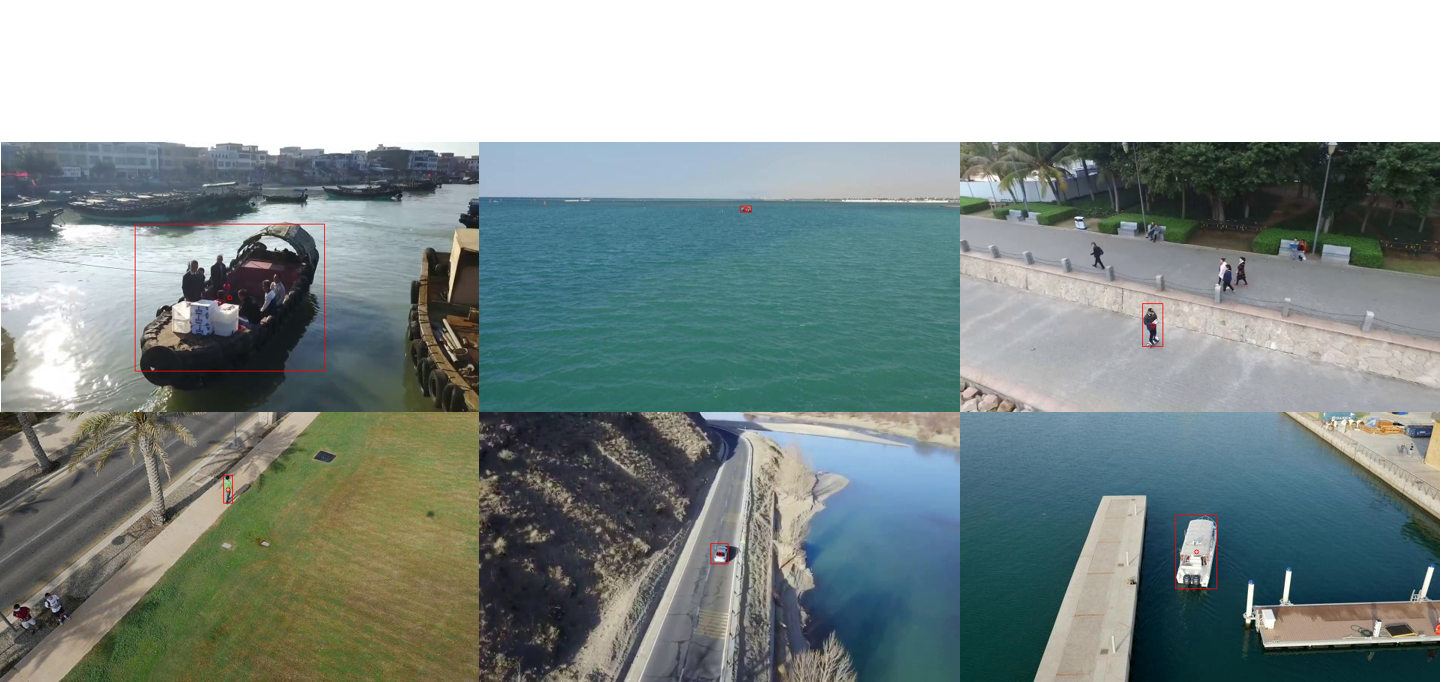
\includegraphics[width=\linewidth]{images/sample_images.png}
    \caption{Przykładowe obrazy zbioru uczącego wraz z zaznaczonymi obiektami detekcji. Źródło \cite{dac_sdc_2021}.}
    \label{fig:sample_images}
\end{figure}

Samo rozwiązanie poddawane jest ocenie danej wzorem \eqref{eq:score}. Uzyskanie wyższej wartości skutkuje uzyskaniem wyższego miejsca w rankingu, z czego wynika, iż funkcję $Score$ należy maksymalizować. 

\begin{equation}
E_{Score} = log_2(E)
\label{eq:e_score}
\end{equation}

\begin{equation}
IoU_{Score} = max(0.1, ReLU(1 - 5 ReLU(0.7 - IoU)))
\label{eq:iou_score}
\end{equation}

\begin{equation}
FPS_{Score} = ReLU(1 - ReLU( 1 - \frac{1}{FPS}))
\label{eq:fps_score}
\end{equation}

\begin{equation}
Score = \frac{10^2}{E_{Score}} IoU_{Score} FPS_{Score}
\label{eq:score}
\end{equation}

Ocenie poddawana jest zarówno dokładność detekcji mierzona współczynnikiem $IoU$ (ang. \emph{Intersection over Union}) na zbiorze tajnym, lecz również przepustowość $FPS$ mierzona poprzez liczbę przetworzonych obrazów na sekundę. 
Ponadto mierzona jest również całkowita energia $E$ zużyta przez układ. 
Zużyta energia jest wyznaczana z iloczynu zmierzonego czasu przetwarzania oraz pomiaru średniej mocy układu. 
Chwilowe wartości mocy są odczytywane z regulatora mocy z częstotliwością próbkowania $20 Hz$.
Zarówno pomiar energii oraz czasu musi być realizowany przez opracowaną aplikację.
Wstępna analiza pozwala stwierdzić, iż uzyskanie wartości $IoU$ oraz $FPS$ poniżej wartości progowych skutkuje zastosowanie kary, natomiast
%nadmierne 
zwiększanie tych wartość powyżej wartości progowych nie przynosi dodatkowych korzyści (przynajmniej w sposób bezpośredni). 

% Analizując wzór \eqref{eq:fps_score} można zauważyć, iż uzyskanie przepustowości powyżej $30 fps$ pozwala na osiągnięcie maksymalnej wartości współczynnika $FPS_{Score}$. Dalsze zwiększenie przepustowości nie zwiększa wartości $FPS_{Score}$. 
% Dla deterministycznego systemu wartość ta powinna być stała. Oczekiwane jest również, iż dla różnych egzemplarzy platformy wartości te będą przyjmowały zbliżoną wartość. Wówczas Funkcja oceny \eqref{eq:score} zależy jedynie od dokładności oraz zużycia energii.

Wśród wymagań znajdują się również informacje odnośnie dostarczenia wymaganych plików.
Aplikacja sterująca ma być zrealizowana w postaci notatnika \emph{Jupyter}.
Dodatkowo należy dostarczyć również pliki \emph{*.hwh} (plik opisu diagramu blokowego logiki programowalnej)
oraz \emph{*.bit} (plik konfiguracji logiki programowalnej) Ponadto należy dołączyć inne niezbędne pliki. 
Finalne rozwiązanie musi być dostępne w formie otwarto-źródłowej.

\section{Platforma sprzętowa}
Ewaluacja wytrenowanej sieci neuronowej jest przeprowadzana na wbudowanej platformie obliczeniowej \emph{Avnet Ultra96-V2} \cite{avnet_ultra96}. Jest to płytka rozwojowa wyposażona w układ \emph{Xilinx Zynq UltraScale+ MPSoC ZU3EG A484}, 2 GB pamięci LPDDR4, slot kart microSD, moduł Wi-Fi, a także porty USB 3.0, porty IO oraz port mini-display. Układ działa pod kontrolą systemu operacyjnego \emph{PetaLinux} wraz z uruchomionym serwerem \emph{Jupyter} (pochodzących z dystrybucji projektu \emph{Pynq}\cite{pynq}). 
Sam układ \emph{Xilinx Zynq UltraScale+ MPSoC ZU3EG A484} jest układem typu SoC. Zawiera czterordzeniowy procesor ARM Cortex-A53 MPCore, dwurdzeniowy procesor Arm Cortex-R5F MPCore oraz procesor graficzny Mali-400 MP2 \cite{zynq_product_guide}. Ponadto układ wyposażony jest w logikę programowalną połączoną z systemem procesorowym magistralą AXI. Logika programowalna zawiera: 154 tys. System Logic Cells, 141 tys. przerzutników oraz 71 tys. LUT (ang. Look-Up Table) zawartych w blokach CLB (ang. Configurable Logic Block), 360 DSP slice, a także 7.6 MB pamięci BRAM. Rysunek \ref{fig:ultra96} przedstawia docelową platformę.

\begin{figure}
    \centering
    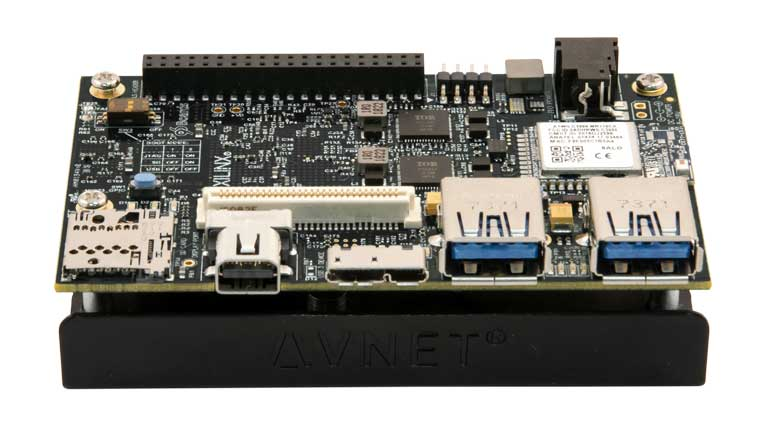
\includegraphics[width=\linewidth]{images/ultra96v2.png}
    \caption{Płytka \emph{Avnet Ultra96 V2}. Źródło \cite{avnet_ultra96}.}
    \label{fig:ultra96}
\end{figure}
 

\section{Przegląd rozwiązań}
Jednym z warunków konkursu jest udostępnienie pełnego rozwiązania w formie otwarto-źródłowej. 
Daje to możliwość analizy rozwiązań z edycji poprzedzających rozpatrywaną.

Zwycięski zespół poprzedniej edycji wykorzystał architekturę sieci \emph{Ultra\_net} \cite{ultra_net}. 
Architektura jest w pełni konwolucyjna (FCNN, ang. Fully Convloutional Neural Network), zawiera 9 warstw kowolucyjnych, warstwy normalizujące (przekształcenie afiniczne) oraz warstwy Max Pooling. 
Ponadto warstwy konwolucyjne zawierały co najwyżej 64 filtry (o wymiarze 3x3) i nie zawierały składowych stałych. Wyjątkiem jest ostatnia warstwa  stanowiąca warstwę typu \emph{YOLOv2}\cite{yolov2} / \emph{Yolov3}\cite{yolov3}, w której składowa stała występuje.
Sprzetowa akceleracja zostałą zrealizowana z użyciem języka HLS (ang. High Level Synthesis). 
Wykorzystano tutaj 4 bitową kwanytyzację wag konwolucji. 
Dla warstw normalizacyjnych kwantyzacja była różna (zależna od położenia warstwy).
Rozwiązanie osiągnęło dokładność detekcji $0.656$ IoU, przepustowość $212.726 fps$ oraz zużyło $1641.1 J$ energii. 

Innym rozwiązaniem jest architektura \emph{SkyNet}\cite{skynet}. 
Przez 3 ostatnie edycje architektura ta osiągała jedne z najlepszych wyników.
Jest to również sieć typu FCNN, wyróżniająca się zastosowaniem konwolucji seperowalnych oraz zastosowaniem funkcji aktywacji $ReLU6$.
W każdym bloku konwolucji separowalnej, po każdej warstwie konwolucji typu depthwise oraz pointwise  występuje warstwa normalizacji z funkcją aktywacji.
Ostatnią warstwę sieci stanowi warstwa \emph{YOLO} (podobnie jak w przypadku \emph{Ultra\_net}).
Ilość filtrów w warstwach oraz położenie warstw Max Pooling zostały zoptymalizowane z użyciem algorytmu PSO.
Rozwiązanie osiągnęło dokładność detekcji $0.716$ IoU, przepustowość $25.05 fps$ oraz zużyło $7260 J$ energii dla implementacji na płytce \emph{Avnet Ultra96 V1}. 

Dotychczas przytoczone rozwiązania wykorzystywały sieci z kwantyzacją wielobitową oraz pochodzące z poprzednich edycji konkursu. Innym podejściem mogącym uzyskać zwiększoną przepustowość oraz mniejsze zużycie energii jest zastosowanie sieci binarnych. Przykładem jest sieć \emph{XNOR-Net}\cite{xnor_net}. Wagi oraz wejścia warstw sieci są poddawane binaryzacji funkcją $sign$. 
Binarne wartości poddawane są binarnej konwolucji, która różni się względem standardowej użyciem funkcji $xor$ zamiast mnożenia. 
Celem poprawienia rezultatów treningu sieci oraz zmniejszenia różnicy pomiędzy odpowiedziami modelu zmiennoprzecinkowego wprowadzono współczynniki skalujące wyznaczane analitycznie. 
Następcą sieci \emph{XNOR-Net} jest sieć \emph{XNOR-Net++}\cite{xnor_net++}. W sieci tej zastąpiono wyznaczane analitycznie współczynniki na rzecz dodatkowych parametrów sieci wyznaczanych w trakcie wstecznej propagacji błędu.
Obie wspomniane sieci binarne były testowane przez autorów dla zadania klasyfikacji. 
Jednakże opisana metodyka może również być zastosowana dla zadania detekcji.


\section{Narzędzia}
Uzyskanie przepustowości $30 fps$, pozwalającej na uzyskanie wysokiej oceny rozwiązania, może być trudne lub nie możliwe do osiągnięcia przy użyciu jedynie części procesorowej nawet dla modeli o niskiej złożoności obliczeniowej. 
Wymagana jest tutaj dodatkowa akceleracja wykorzystująca logikę programowalną. 
W tym celu możliwe jest wykorzystanie istniejących narzędzi wspomagających sprzętową implementację, a także proces uczenia. 

Uczenie sieci z przeznaczeniem do sprzętowej akceleracji zazwyczaj wiąże się z wytrenowaniem modelu zmiennoprzecinkowego, następnie jego kwantyzacji oraz finalnie implementacji sprzętowej.
Etap wytrenowania modelu zmiennoprzecinkowego może zostać przeprowadzony z użyciem dowolnych narzędzi, narzędzi wspieranych na dalszych etapach lub konwersji modelu do wspieranego formatu. 
Następnym etapem jest kwantyzacja. Na tym etapie wagi oraz wyniki pośrednie warstw sieci są poddawane kwantyzacji. 
Zazwyczaj wyniki sieci kwantyzowanej różnią się od wyników modelu zmiennoprzecinkowego, przez co wymagane jest wznowienie procesu uczenia.
Daje to możliwość pominięcia treningu modelu zmiennoprzecinkowego.
Model kwantyzowany możliwy jest do sprzętowej implementacji z wykorzystaniem wybranych narzędzi.

Poniżej wymieniono wybrane narzędzia wspomagające sprzętową implementację. 
\begin{itemize}
    \item \emph{Brevitas}\cite{brevitas} - biblioteka dla frameworka \emph{PyTorch}\cite{pytorch}, przeznaczona do wspomagania kwantyzacji i treningu QNN. Biblioteka rozwijana przez \emph{Xilinx}.
    
    \item \emph{FINN}\cite{finn} - framework rozwijany przez \emph{Xilinx} pozwalający na implementację sprzętową QNN w typie przetwarzania potokowego.
    
    \item \emph{QKeras}\cite{qkeras} - biblioteka dla frameworka \emph{TensorFlow}\cite{tf} pozwalająca na kwantyzację i trening QNN.
    \item \emph{hls4ml}\cite{hls4ml} - biblioteka dokonująca konwersji modelu QNN do zapisu z użyciem języka HLS. 
    
    \item \emph{Vitis AI}\cite{vitis_ai} - środowisko pozwalające na przeprowadzenie kwantyzacji, optymalizacji architektury sieci oraz sterowania procesem akceleracji poprzez stosowne biblioteki C++/Python. Jest to środowisko rozwijane przez firmę \emph{Xilinx}
    Wykorzystywana jest tutaj akceleracja z wykorzystaniem generycznego  DPU (ang. Deep Processing Unit) możliwego do konfiguracji.
    
\end{itemize}


W analizę problemu włączono zarówno wymagania konkursowe, dostępną platformę sprzętową, a także istniejące rozwiązania i narzędzia.
Głównym celem jest implementacja szybkiego i energooszczędnego rozwiązania, pozwalającego na dokładną detekcję pojedynczych obiektów. 
Zadanie jest realizowane w oparciu o sprzętową akcelerację wykorzystującą logikę programowalną płytki \emph{Avnet Ultra96 V2}.
Dostępnych jest wiele bibliotek usprawniających proces kwantyzacji, jak również implementacji sprzętowej.
Możliwe jest wykorzystanie lub wzorowanie się na istniejących już rozwiązaniach zapewniających wysoką przepustowość oraz niskie zużycie energii. 


% Należy zaznaczyć, iż architektury sieci przed i po procesie kwantyzacji nie mogą lub nie powinny być rozważanie jako identyczne ze względu na znaczne zmiany jakie wprowadza kwantyacja.  


%---------------------------------------------------------------------------

    


	\chapter{Badania wstępne}
\label{cha:Badania wstępne}

Analiza rozpatrywanego problemu detekcji wraz ze sprzętową implementacją pozwala na zaproponowanie możliwych rozwiązań. W niniejszym rozdziale zostaną przedstawione propozycje architektur sieci, proces ich uczenia a także kwantyzacji. 

\section{Architektura wstępna} %section{Architektura wstępna}

%}
% Liczba parametrów sieci \emph{Ultra\_net} wynosi ponad 200 tys..
Liczba parametrów sieci \emph{SkyNet}\footnote{W wersji bez połączenia typu \emph{bypass}} wynosi ponad $300$ tys. 
Zastosowanie separowalnych konwolucji skutkuje znaczną redukcją liczby parametrów względem architektury wykorzystującej pełną konwolucję - powyżej $2.6$ miliona parametrów \footnote{Architektur tych nie można w pełni ze sobą utożsamiać jako substytutów.}. 
Tak znaczna redukcja (również złożoności obliczeniowej) skłania do zastosowania konwolucji separowalnych dla sprzętowej akceleracji. 
W tym celu rozważono architekturę sieci o 9 warstwach konwolucji separowalnej (z bias) z funkcją aktywacji $ReLU$ po konwolucji typu pointwise. Architektura posiada również warstwy Max Pooling po każdej konwolucji separowalnej.
Ostatnia warstwa stanowi warstwę podobną do warstwy \emph{YOLOv1}. Na rysunku \ref{fig:arch_v1} przedstawiono graficzną reprezentację architektury. 
Jako wejście sieci pozostawiono oryginalne wymiary obrazów dostępnych w zbiorze treningowym.

Ze względu, iż rozpatrywany problem to detekcja bez klasyfikacji, pominięto w funkcji błędu \eqref{eq:lossv1} część związaną z klasyfikacją. 
Jako wartości referencyjne dla wyjść sieci wykorzystano maskę $y_{ref}$ (o wymiarach 5x7x12) z odpowiadającymi wartościami dla kanałów. Równania \eqref{eq:y_ref_valv1}-\eqref{eq:y_ref_hv1} prezentują sposób wyznaczenia wartości referencyjnych dla elementów poszczególnych kanałów. 

\begin{figure}
    \centering
    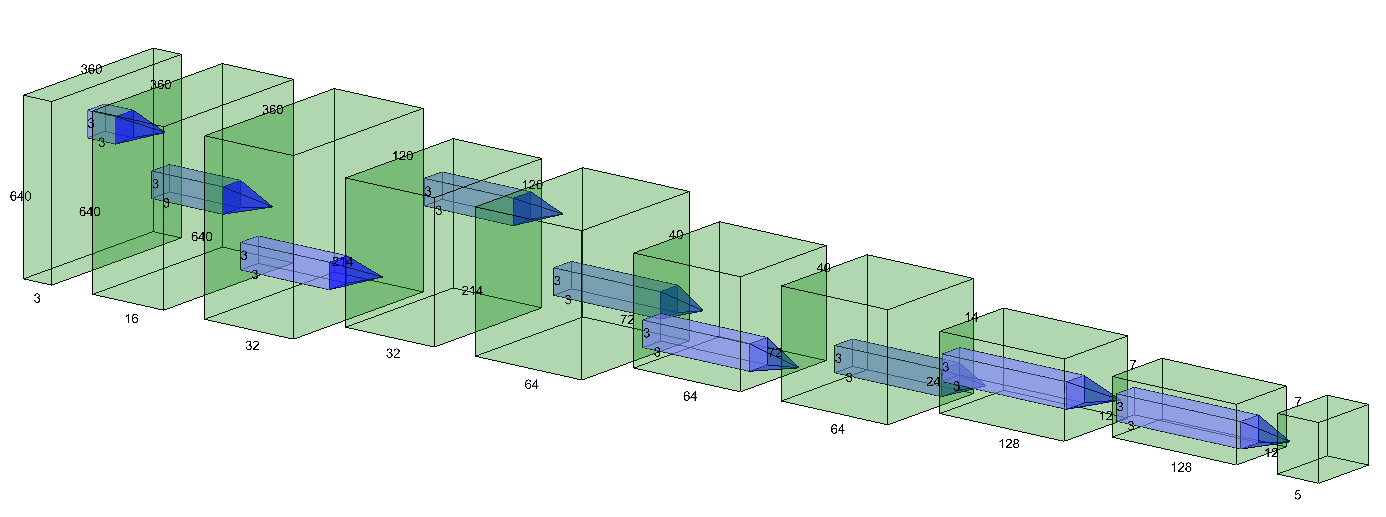
\includegraphics[width=\linewidth]{images/arch_v1.png}
    \caption{Wstępna architektura sieci dla zadania detekcji, wykorzystująca konwolucje separowalne oraz warstwę podobną do \emph{YOLOv1}. Architektura posiada niespełna 43 tys. parametrów.}
    \label{fig:arch_v1}
\end{figure}

\begin{equation}
y_{ref}_{0,i,j} = 
\begin{cases}
    1, & \text{if }  i = row \And j = col \\
    0,              & \text{otherwise}
\end{cases}
\label{eq:y_ref_valv1}
\end{equation}

\begin{equation}
y_{ref}_{1,i,j} = 
\begin{cases}
    x_c \frac{12}{640} - col - 0.5, & \text{if }  i = row \And j = col \\
    0,              & \text{otherwise}
\end{cases}
\label{eq:y_ref_xv1}
\end{equation}

\begin{equation}
y_{ref}_{2,i,j} = 
\begin{cases}
    y_c \frac{7}{360} - row - 0.5, & \text{if }  i = row \And j = col \\
    0,              & \text{otherwise}
\end{cases}
\label{eq:y_ref_yv1}
\end{equation}

\begin{equation}
y_{ref}_{3,i,j} = 
\begin{cases}
    log(\frac{w}{a_w}) & \text{if }  i = row \And j = col \\
    0,              & \text{otherwise}
\end{cases}
\label{eq:y_ref_wv1}
\end{equation}

\begin{equation}
y_{ref}_{4,i,j} = 
\begin{cases}
    log(\frac{h}{a_h}) & \text{if }  i = row \And j = col \\
    0,              & \text{otherwise}
\end{cases}
\label{eq:y_ref_hv1}
\end{equation}

$row$ oraz $col$ oznaczają indeks siatki wyjściowej do którego został przypisany referencyjny obiekt, $a_w$ oraz $a_h$ odpowiednio szerokość i wysokość \emph{anchor box}. 
Przyjęto  $a_w = 16$ oraz $a_h = 16$ jako wartość łączna wartość kroku sieci (ang. \emph{stride}) wynikająca z liczby warstw Max Pooling.
Przyjmując za $x_c, y_c, w, h$ odpowiednio współrzędne położenia środka obiektu oraz jego wymiary, można wyznaczyć indeksy $row$ oraz $col$ według wzorów \eqref{eq:rowv1}-\eqref{eq:colv1}.

\begin{equation}
col = \round{x_c \frac{12}{640} - 0.5}
\label{eq:colv1}
\end{equation}
\begin{equation}
row = \round{y_c \frac{7}{360} - 0.5}
\label{eq:rowv1}
\end{equation}


Błąd wykrycia obiektu został zdefiniowany jako entropia binarna $BCE$. 
Błąd przesunięcia od centrum siatki detekcji (wynikającej z wymiarów ostatniej warstwy) został zdefiniowany jako średni błąd bezwzględny $MAE$. Błąd wymiarów został zdefiniowany jako wartość średnia pierwiastka $MSQRT$ z wartości bezwzględnej różnicy pomiędzy odpowiedzią sieci oraz wartością referencyjną.
Funkcję błędu (reprezentowaną przez równanie \eqref{eq:lossv1}) dla całej sieci stanowi ważona suma błędów składowych ze współczynnikami $\lambda_obj, \lambda_xy oraz \lambda_wh$. 

\begin{equation}
\begin{aligned}
loss =& \lambda_{obj} BCE(\sigma(y_{pred}_{0,:,:}), y_{ref}_{0,:,:}) \\
&+ \frac{\lambda_{xy}}{2}( MAE(y_{pred}_{1,:,:}, y_{ref}_{1,:,:}) + MAE(y_{pred}_{2,:,:}, y_{ref}_{2,:,:})) \\
&+ \frac{\lambda_{wh}}{2} (MSQRT(|y_{pred}_{3,:,:} - y_{ref}_{3,:,:}|) + MSQRT(|y_{pred}_{4,:,:} - y_{ref}_{4,:,:}|))
\end{aligned}
\label{eq:lossv1}
\end{equation}


Przed rozpoczęciem procesu uczenia dokonano podziału dostępnego zbioru uczącego na trzy zbiory: uczący, walidacyjny oraz testowy w stosunku 81:9:10. Podział został przeprowadzony losowo wewnątrz każdej sekwencji.
Uzyskany podział zbioru był stosowany dla wszystkich dalszych wariantów architektur i funkcji błędu.

Rozpoczynając trening sieci ustalono wszystkie parametry funkcji błędu \eqref{eq:lossv1} na wartość $1$.
Dla zbioru uczącego przeprowadzano augmentację danych\footnote{Dla pozostałych wariantów architektur również przeprowadzano augmentację danych.} z wykorzystaniem filtracji uśredniającej, zakłóceń addytywnych, przeskalowania czy też rotacji.
Do minimalizacji błędu użyto algorytmu \emph{Adadelta}\footnote{Dla pozostałych architektur również użyto tego algorytmu.}.

Proces uczenia przerwano, gdy nie zauważono zmian wartości błędu oraz metryki IoU dla zbioru uczącego oraz walidacyjnego.
Finalnie architektura osiągnęła wartość współczynnika $iou = 0.47$ dla zbioru walidacyjnnego.

\section{Architektura rozgałęziona}
Ze względu na niewielką wartość współczynnika $iou$, architekturę zmodyfikowano o dodanie dodatkowego wyjścia z sieci pochodzącego z warstwy pośredniej zakończonego warstwą analogicznie do wersji nierozgałęzionej (wymiary \emph{anchor box} dla rozgałęzienia $a_w = 8$ oraz  $a_h = 8$). Na rysunku \ref{fig:arch_v2} przedstawiono graficzną reprezentację architektury. Po przeprowadzeniu procesu ucznia sieci, z wykorzystaniem techniki transferu wiedzy z architektury pierwotnej, uzyskano pogorszenie wartości $iou$. 

\begin{figure}
    \centering
    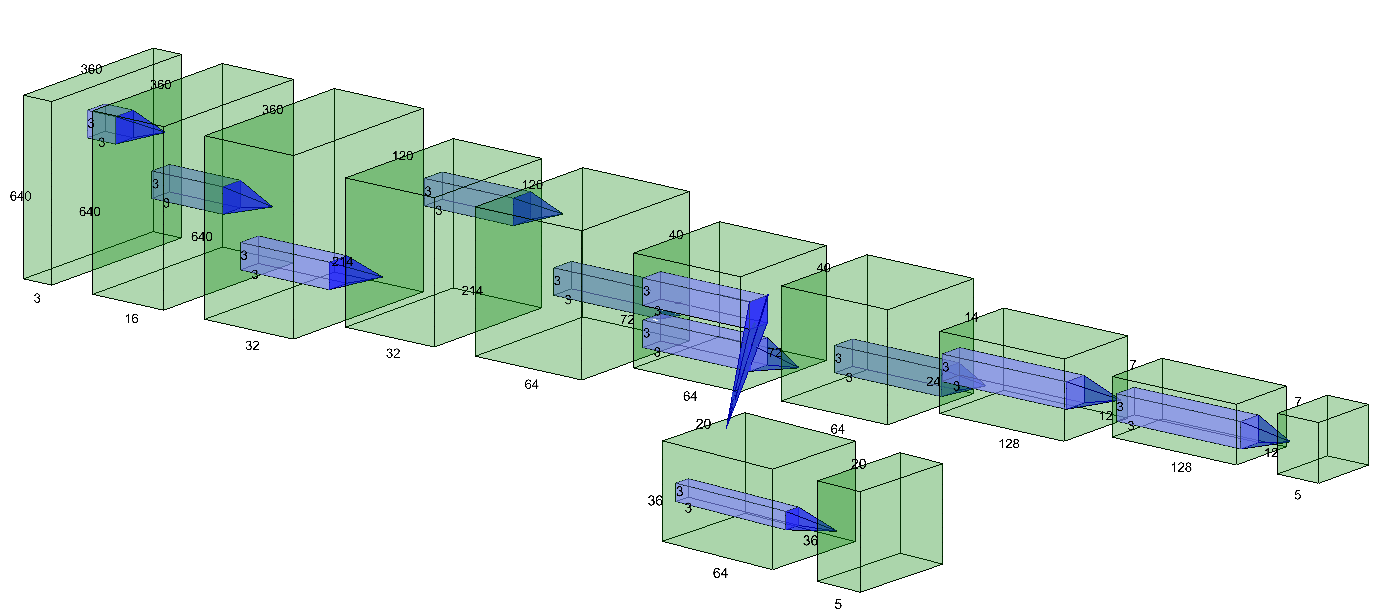
\includegraphics[width=\linewidth]{images/Architektura_branched.png}
    \caption{Architektura rozgałęziona wykorzystująca konwolucje separowalne.}
    \label{fig:arch_v2}
\end{figure}


\section{Architektura Resnet18}
Rezultaty dotychczas badanych architektur były niewystarczające. Rozważono wówczas architekturę wykorzystującą połączenia residualne - \emph{Resnet18}\cite{resnet18}. 
W tym celu wykorzystano dwa pierwsze bloki residualne (sieci przetrenowanej na zbiorze danych \emph{ImageNet}\cite{imagenet} dostępnej za pośrednictwem biblioteki \emph{PyTorch}) oraz dodano warstwę \emph{Yolov2}\cite{yolov2} poprzedzoną warstwą konwolucyjną ze 128 filtrami. 
Wykorzystano tu trzy \emph{anchor box} o wymiarach(szerokość x wysokość): $22x33, 43x69, 89x133$ uzyskanych jako wynik algorytmu k-średnich. 
Uzyskana architektura podsiadała ponad 700 tys. paramterów.
Wymiary obrazów wejściowych zredukowano do 360 pikseli szerokości oraz 180 pikseli wysokości.
Funkcja błędu odpowiedzi sieci przyjmuje postać daną równaniem \eqref{eq:loss_yolo_v2}.
Jako funkcję błędu regresji $loss_{bbox}$ wybrano funkcję \emph{GIoU}\cite{giou}. Dla błędu wykrycia obiektu zastosowano (podobnie jak dla poprzednich architektur) entropię binarną. Dla obu współczynników wagowych przyjęto wartość $1$.
\begin{equation}
loss = \lambda_{validity} BCE(y_{pred}_{0:2,:,:}, y_{ref}_{0:2,:,:}) + \lambda_{bbox} loss_{bbox}(y_{pred}_{3:14,:,:}, x_c,y_c,w,h)
\label{eq:loss_yolo_v2}
\end{equation}


Dla modelu zmiennoprzecinkowego architektura osiągnęła wartość $iou$ ponad $0.8$ dla zbioru walidacyjnego. Proces uczenia został przerwany podobnie jak poprzednio, gdy nie zauważano znacznych zmian błędu i metryki \emph{IoU}.

Zdecydowano się na kwantyzację modelu z wykorzystaniem zapisu stałoprzecinkowego. 
Obraz wejściowy został poddany kwantyzacji 8 bitowej bez znaku i bez części całkowitej. 
Wagi oraz wyjścia warstw pośrednich poddano kwantyzacji 8 bitowej ze znakiem i 2 bitami części całkowitej.
Ostanie dwie warstwy poddano kwantyzacji 8 bitowej ze znakiem i 3 bitami części całkowitej.
W przypadku każdej kwantyzacji zastosowano również ograniczenie wartości wynikowej do limitów wynikających z zapisu w formacie stałoprzecinkowym.

Następnie po zakończeniu treningu sieci z kwantyzacją osiągnięto wartość $iou = 0.72$.
Uzyskana wartość pozwalałaby na osiągnięcie maksymalnej wartości oceny\footnote{Jeżeli uzyskano by podobny rezultat na zbiorze tajnym.} danej równaniem \eqref{eq:iou_score}. 

Rozważana architektura wydaje się być trudniejsza do sprzętowej implementacji ze względu na połączenia residualne oraz znaczne rozmiary. 
Jednakże analizując przeprowadzone procesy uczenia można zauważyć, iż dodanie warstw normalizujących oraz zastosowanie funkcji błędu bazującej na metryce \emph{IoU} pozwala na osiągnięcie większych wartości \emph{IoU}, przy mniejszej liczbie epok treningowych \footnote{Dla poprzednich architektur liczba epok była znacznie większa, niż dla architektury residualnej}. 


\section{LittleNet}

Podsumowując wnioski z rozważanych dotychczas architektur można stwierdzić, iż:
\begin{itemize}
    \item zastosowanie konwolucji separowalnych pozwala na znaczną redukcję liczby parametrów oraz złożoności obliczeniowej, 
    \item warstwy normalizacji pozwalają zmniejszyć liczbę epok treningowych,
    \item funkcja błędu bazująca na matryce \emph{IoU} pozwala osiągnąć lepsze wyniki.
\end{itemize}

Dodatkowo można zauważyć, konwolucja separowalna dla pierwszej warstwy posiada jedynie trzy filtry typu depthwise.
Następna warstwa typu pointwise dokonuje podziału w przestrzeni zaledwie trójwymiarowej. 
Może to skutkować pewną utratą znacznej części informacji już na początkowym etapie przetwarzania, a także pewną redundancją filtrów pointwise lub ich wrażliwości na nie wielkie zmiany wejścia. 
Zastosowanie pełnej konwolucji w pierwszej warstwie mogłoby polepszyć jakość detekcji.
Jednakże kownolucje pełne są bardziej złożone w implementacji sprzętowej. 
Z tego względu zdecydowano się na zastosowanie wielokrotnej filtracji typu depthwise. 
Pozwala to na zwiększenie liczby cech bezpośrednio ekstrahowanych z obrazu wraz z zachowaniem możliwości stosunkowo łatwej implementacji sprzętowej.

Proponowaną architekturę przedstawiono na rysunku \ref{fig:LN_arch}. 
Sieć zawiera 7 bloków z konwolucją typu depthwise oraz 7 z konwolucją typu pointwise. Po każdej konwolucji występuje warstwa normalizacyjna oraz funkcja aktywacji $ReLU$. Pierwszy blok zawiera warstwę depthwise posiada z 5 filtrami na kanał, kolejne bloki zawierają już tylko po 2 filtry na kanał.
Po pierwszych 4 warstwach pointwise  występuje warstwa Max Pooling. 
Ostatnią warstwę stanowi konwolucja typu pointwise stanowiąca warstwę \emph{YOLOv2}. Wymiary \emph{anchor box} pozostały takie same jak dla architektury wykorzystującej bloki residualne, lecz przeskalowane do wymiarów wejścia sieci. 
Proponowana architektura posiada niespełna 134 tys. parametrów, co stanowi znaczą redukcję liczby parametrów w stosunku do \emph{SkyNet} (powyżej 300 tys.) oraz \emph{Ultra\_net} (ponad 200 tys.). 
Architekturze nadano % roboczą
nazwę \emph{LittleNet}.
\begin{figure}
    \centering
    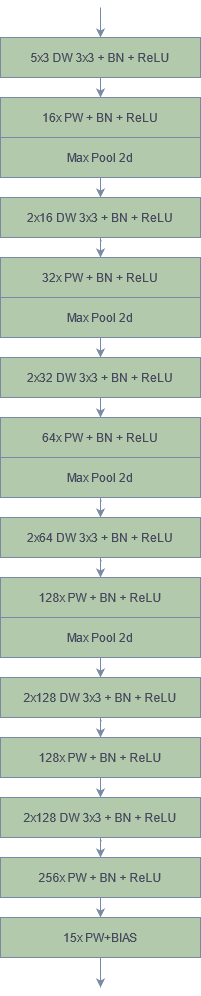
\includegraphics[width=4cm]{images/LNv1}
    \caption{Proponowana architektura sieci \emph{LittleNet}.}
    \label{fig:LN_arch}
\end{figure}

Rozmiar wejścia sieci ustalono na 360 pikseli szerokości oraz 180 pikseli wysokości.
Funkcja błędu odpowiedzi sieci \eqref{eq:loss_yolo_v2} rozszerzono o regularyzację normą $L_1$ parametrów sieci $p$, uzyskując równanie \eqref{eq:loss_yolo_v2_reg}. .
\begin{equation}
\begin{aligned}
loss =& \lambda_{validity} BCE(y_{pred}_{0:2,:,:}, y_{ref}_{0:2,:,:}) \\
&+ \lambda_{bbox} loss_{bbox}(y_{pred}_{3:14,:,:}, x_c,y_c,w,h)\\
&+ \lambda_{reg} L_1(p)
\end{aligned}
\label{eq:loss_yolo_v2_reg}
\end{equation}
Za funkcję błędu regresji $loss_{bbox}$  przyjęto funkcję \emph{GCIoU} daną równaniem \eqref{eq:gciou}. 
Funkcja ta bazuje na \emph{GIoU}\cite{giou}, \emph{DIoU}\cite{dciou} oraz \emph{CIoU}\cite{dciou}. 
Połączenie powyższych funkcji pozwala na połączenie ich zalet funkcji: 
\begin{itemize}
    \item \emph{GIoU} - bardziej bezpośredni wpływ błędu na parametry (gdy \emph{IoU}$ = 0$),
    \item \emph{DIoU} - centralizacji predykcji,
    \item \emph{CIoU} - wzmocnione finalne skalowanie rozmiaru. 
\end{itemize}
\begin{equation}
GCIoU = GIoU + CIoU + IoU - 1
\label{eq:gciou}
\end{equation}
Ustalono parametry wagowe na $\lambda_{validity} = 20$, $\lambda_{bbox} = 1$ oraz $\lambda_{reg} = 0.01$.
Krok uczący został początkowo ustalony jako $l_r=1$. 
W trakcie procesu uczenia podlegał on modyfikacją zgodnie z równaniami \eqref{eq:lr_1} oraz \eqref{eq:lr_2}.
\begin{equation}
l_r_(t+1) = 
\begin{cases}
    1.3*l_r(t), &\text{if } loss(t) < loss(t-1) \\
    0.5*l_r(t), &\text{if } loss(t) > loss(t-1) \\
    l_r(t), &\text{otherwise}
\end{cases}
\label{eq:lr_1}
\end{equation}
\begin{equation}
l_r(t+1) = max(10^{-5}, min(1, l_r(t+1)))
\label{eq:lr_2}
\end{equation}


Po zakończeniu procesu uczenia modelu zmiennoprzecinkowego osiągnięto wartość $iou = 0.8$ dla zbioru walidacyjnego oraz $0.7$ dla zbioru uczącego. 
Powodem tak znacznej różnicy wartości metryki jest znaczny stopień augmentacji danych.

Sieć poddano kwantyzacji. Dane wejściowe zostały poddane kwantyzacji 8 bitowej bez znaku i bez części całkowitej.
Warstwy pośrednie poddano kwantyzacji 8 bitowej ze znakiem i 2 bitami części całkowitej.
Ostatnią warstwę poddano kwantyzacji 8 bitowej ze znakiem i 3 bitami części całkowitej.

Uzyskano wartość $iou = 0.76$ dla zbioru walidacyjnego oraz $0.67$ dla zbioru uczącego.
Na rysunkach \ref{fig:float_loss}-\ref{fig:quant_iou} przedstawiono przebiegi funkcji błędu oraz metryki \emph{IoU} dla modelu zmiennoprzecinkowego oraz kwantyzowanego.

\begin{figure}
     \centering
     \begin{subfigure}[b]{0.49\textwidth}
         \centering
         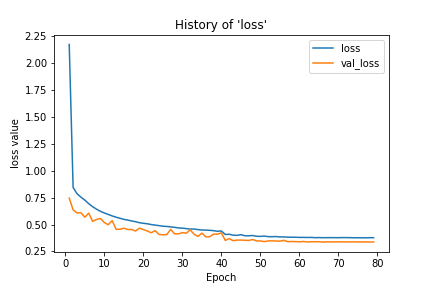
\includegraphics[width=\textwidth]{images/float32_hist_of_loss.png}
         \caption{}
         \label{fig:float_loss}
     \end{subfigure}
     \hfill
     \begin{subfigure}[b]{0.49\textwidth}
         \centering
         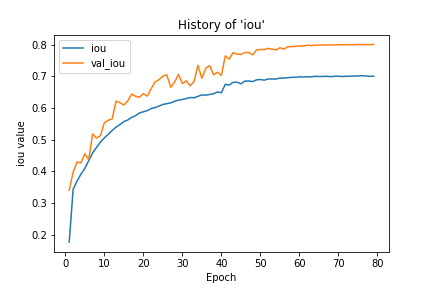
\includegraphics[width=\textwidth]{images/float32_hist_of_iou.png}
         \caption{}
         \label{fig:float_iou}
     \end{subfigure}
     \hfill
     \begin{subfigure}[b]{0.49\textwidth}
         \centering
         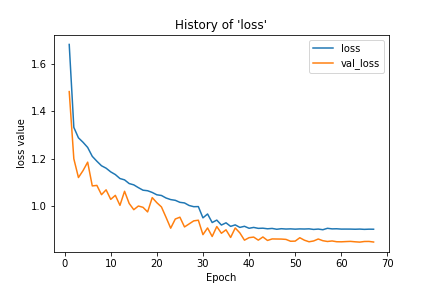
\includegraphics[width=\textwidth]{images/8_bit_quant_hist_of_loss.png}
         \caption{}
         \label{fig:quant_loss}
     \end{subfigure}
     \hfill
     \begin{subfigure}[b]{0.49\textwidth}
         \centering
         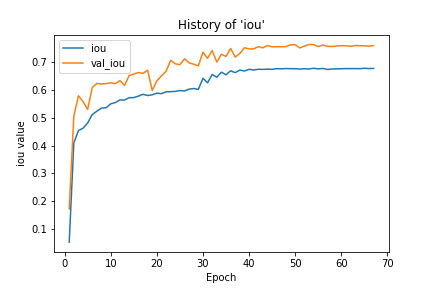
\includegraphics[width=\textwidth]{images/8_bit_quant_hist_of_iou.png}
         \caption{}
         \label{fig:quant_iou}
     \end{subfigure}
     \hfill
     
    \caption{Przebiegi wartości błędu oraz metryki \emph{IoU} (w zależności od epoki uczącej) dla modelu zmiennoprzecinkowego \ref{fig:float_loss} i \ref{fig:float_iou} oraz \ref{fig:quant_loss} i \ref{fig:quant_iou}.}
    \label{fig:two_step_train}
\end{figure}


W trakcie realizacji implementacji sprzętowej, ustalono, iż dla obecnego rozmiaru wejścia sieci nie jest możliwe buforowanie wyników warstw pośrednich w pamięci BRAM.
Z tego względu zdecydowano się na redukcję rozmiaru wejścia sieci do 200 pikseli szerokości oraz 100 pikseli wysokości. 
Rozpoczęto trening sieci z takimi samymi parametrami (wagi sieci zostały wylosowane).  
Uzyskano wartość $iou = 0.78$ dla zbioru walidacyjnego oraz $0.69$ dla zbioru uczącego.
Od epoki $75$ rozpoczęto kwantyzację z wyłączeniem warstw normalizujących.
Względem poprzedniego modelu zmieniono liczbę bitów części całkowitej: 1 dla wyjść oraz 3 dla wag warstw pośrednich.
Następnie od epoki $109$ kwantyzacji poddano również warstwy normalizujące.
Dla modelu w pełni kwantyzowanego uzyskano wartość $iou = 0.71$ dla zbioru walidacyjnego oraz $0.64$ dla zbioru uczącego. Na rysunkach \ref{fig:small_loss}-\ref{fig:small_iou} przedstawiono przebiegi funkcji błędu oraz metryki \emph{IoU} dla modelu o zmniejszonych rozmiarach wejścia. 

\begin{figure}
     \centering
     \begin{subfigure}[b]{0.49\textwidth}
         \centering
         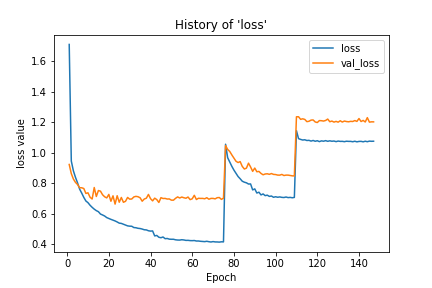
\includegraphics[width=\textwidth]{images/LN_smaller_hist_of_loss.png}
         \caption{}
         \label{fig:small_loss}
     \end{subfigure}
     \hfill
     \begin{subfigure}[b]{0.49\textwidth}
         \centering
         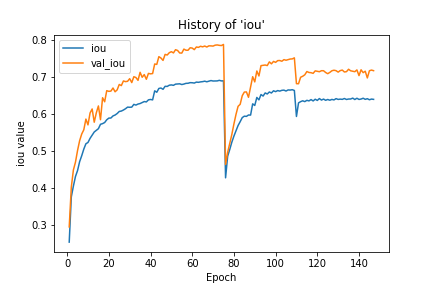
\includegraphics[width=\textwidth]{images/LN_smaller_hist_of_iou.png}
         \caption{}
         \label{fig:small_iou}
     \end{subfigure}
     
    \caption{Przebiegi wartości błędu \ref{fig:small_loss} oraz metryki \emph{IoU} \ref{fig:small_iou} (w zależności od epoki uczącej) dla modelu o rozmiarze wejścia 200x100 pikeli.
    Epoka 75 - rozpoczęcie kwantyzacji bez warstw normalizacyjnych. Epoka 109 - pełna kwantyzacja.}
    \label{fig:three_step_train}
\end{figure}


%  Podsumowanie
Poprzez analizę przeprowadzonych badań architektury stwierdzono, iż stosowanie konwolucji separowalnych posiada zaletę w postaci stosunkowo nie wielkiej liczby parametrów, lecz również wadę wynikającą ze stosunkowo niewielkiego stopnia ekstrakcji cech z danych wejściowych (w szczególności w warstwach początkowych). 
Problem ten rozwiązano poprzez wielokrotną filtrację filtrami typu depthwise.
Ponadto zastosowanie warstw normalizacyjnych pozwoliło na przyspieszenie procesu uczenia.
Wykorzystując wnioski z przeprowadzonych badań zaprojektowano architekturę \emph{LittleNet}. 
Osiągnięto dokładność $iou = 0.71$ wraz ze stosunkowo łatwą implementacją sprzętową.
	\chapter{Implementacja}
\label{cha:Implementacja}
Opis implementacji zarówno programowej jak i sprzętowej.



	\chapter{Implementacja programowa oraz sprzętowa wybranej architektury sieci}
\label{cha:Implementacja}
% Opis oraz omówienie implementacji zarówno programowej jak i~sprzętowej.

Opracowanie odpowiedniej architektury sieci oprócz rozważań teoretycznych, wymagało również wykonania szeregu eksperymentów obliczeniowych.
Ponadto konieczna była implementacja sprzętowa modelu celem akceleracji obliczeń zaprojektowanej architektury na wybranej platformie obliczeniowej.

\section{Implementacja programowa}

Implementacja programowa została zrealizowana w~ramach framework'a \emph{PyTorch} \cite{pytorch}.
Wykorzystano również bibliotekę \emph{Brevitas} \cite{brevitas} do realizacji odpowiedniej metody kwantyzacji.
Metodyka implementacji kwantyzacji opiera się o~klasę \emph{ExtendedInjector}.
Pozwala ona na ``wstawienie'' operacji kwantyzacji wag bezpośrednio przed zastosowaniem ich w~obliczeniach.
Ponadto biblioteka rozszerza predefiniowane w~\emph{PyTorch} warstwy o~operacje kwantyzacji. 
W wersji kwantyzowanej dostępne są m.in. warstwa konwolucji, \emph{Max Pooling} czy funkcja $ReLU$.
Kwantyzowana warstwa normalizacji została zdefiniowana jako przekształcenie afiniczne bez aproksymacji średniej i~wariancji.
Wymagało to implementacji własnej warstwy dokonującej wyboru pomiędzy warstwą zmiennoprzecinkową oraz jej wersją kwantyzowaną.
Augmentacja danych została zrealizowana w~oparciu o~bibliotekę \emph{OpenCV} \cite{opencv}.
Obliczenia były wykonywane na platformie \emph{GoogleColab} \cite{colab} z~wykorzystaniem \emph{GPU}.
Ze względu, iż dzienny czas użytkowania usługi jest ograniczony wymagane było przechowywanie stanu procesu ucznia w~plikach zapisywanych poprzez usługę \emph{GoogleDrive}.


Dla celu testowania wyników implementacji sprzętowej poszczególnych warstw został zaimplementowany dodatkowy model programowy (dwóch typów warstw). 
Wykorzystywał on obliczenia całkowitoliczbowe do wykonania operacji konwolucji \emph{DW} oraz \emph{PW}.
Ponadto zaimplementowano także konwersję wag zmiennoprzecinkowych do stałoprzecinkowych wymaganych do inicjalizacji pamięci ROM akceleratorów opisanych w~dalszej części.

\section{Implementacja sprzętowa}

Wstępnie planowano implementacje sprzętową z~wykorzystaniem narzędzia \emph{FINN} \ref{ch:tools}.
Jednakże ze względu na braki w~dokumentacji (np. implementacja własnej metody kwantyzacji w~\emph{Brevitas}), a~także brak możliwości akceleracji warstwy \emph{BN} (przynajmniej bezpośrednio) zdecydowano się na implementację własną.
Początkowo w~języku wysokopoziomowym \emph{HLS}, lecz ostatecznie w~języku opisu sprzętu \emph{System Verilog}
%, uzyskując w ten sposób pełną kontrolę sposobem implementacji
.
Akceleracja całej sieci stanowi architekturę potokową gruboziarnistą (ang. \emph{coarse grained}).
Schemat przedstawiono na rysunku \ref{fig:LNACC}.
Na elementy wspomnianej architektury składają się:
\begin{description}
\item  bloki komunikacji - realizują wymianę danych z~\emph{DMA} (ang. \emph{Direct Memory Access}) \cite{dma} poprzez magistralą \emph{AXI4-Stream} \cite{axis}. 
Blok \emph{AXIS RECEIVER} odbiera i przekształca strumień danych do postaci wymaganej na dalszym etapie. Wysyłanie danych odbywa się poprzez blok \emph{AXIS SENDER}.
\item \emph{IL} (ang. \emph{Input Layer}) - warstwa wejściowa zmiana formatu danych wejściowych.
\item \emph{ROM}(ang. \emph{Read-Only Memory}) - przechowywanie wag poszczególnych warstw.
\item \emph{RAM})(ang. \emph{Random Access Memory}) - przechowywanie danych wejściowych oraz rezultatów poszczególnych akceleratorów.
\item multipleksery - zarządzanie dostępem do pamięci.
\item \emph{DW, PW, BN, MP, B} - bloki akceleratorów warstw w zadanych konfiguracjach.
Poszczególne akceleratory pogrupowane są po 3 w~bloku. 
Na jeden blok przypisane są dwa bloki pamięci RAM, w~tym jeden z~dostępem  multipleksowanym.
Ma to na celu ograniczenie wymaganej pamięci, kosztem zmniejszenia przepustowości. 
\item \emph{SSR} - rejestr szeregowo-równoległy (ang. \emph{Serial-Parallel Register}) realizuje odbiór danych z ostatniej warstwy.
\item \emph{LN\_CU} (ang. \emph{LittleNet Control Unit}) -  logika sterująca procesem akceleracji.
\end{description}

% Na elementy wspomnianej architektury składają się bloki komunikacji zewnętrznej, pamięci RAM oraz ROM, multipleksery dostępu do pamięci, akceleratory poszczególnych warstw oraz logika sterująca (\emph{LN\_CU}, ang. \emph{LittleNet Control Unit}).
% Wykorzystywana jest tutaj komunikacja z~wykorzystaniem protokołu \emph{AXI4-Stream} \cite{axis} do komunikacji z~\emph{DMA} (ang. \emph{Direct Memory Access}) \cite{dma}.
% Wymiana danych odbywa się za pośrednictwem  modułów \emph{AXIS RECEIVER} do odbioru oraz \emph{AXIS SENDER} do wysyłania danych zgromadzonych w~rejestrze \emph{SPR} (ang. \emph{Serial-Parallel Register}).

Proces akceleracji odbywa się według schematu prezentowanego w~tabeli \ref{tab:LNACC}.
Zostało to zrealizowane w postaci maszyny stanów.
W danym stanie 0-3 aktywne są akceleratory 0-2 z bloków 0-5, dla których występuje wartość 1.
W tabeli \ref{tab:LNACC} oznaczono również typy każdego akceleratora.
Pozwala to uzyskać ciąg operacji przetwarzania danych tożsamy z architekturą sieci. 
W jednej chwili są aktywne akceleratory co czwartej warstwy.
Jest to wymagane, aby udzielić dostępu do wybranych bloków pamięci kilku akceleratorom.

\begin{figure}
    \centering
    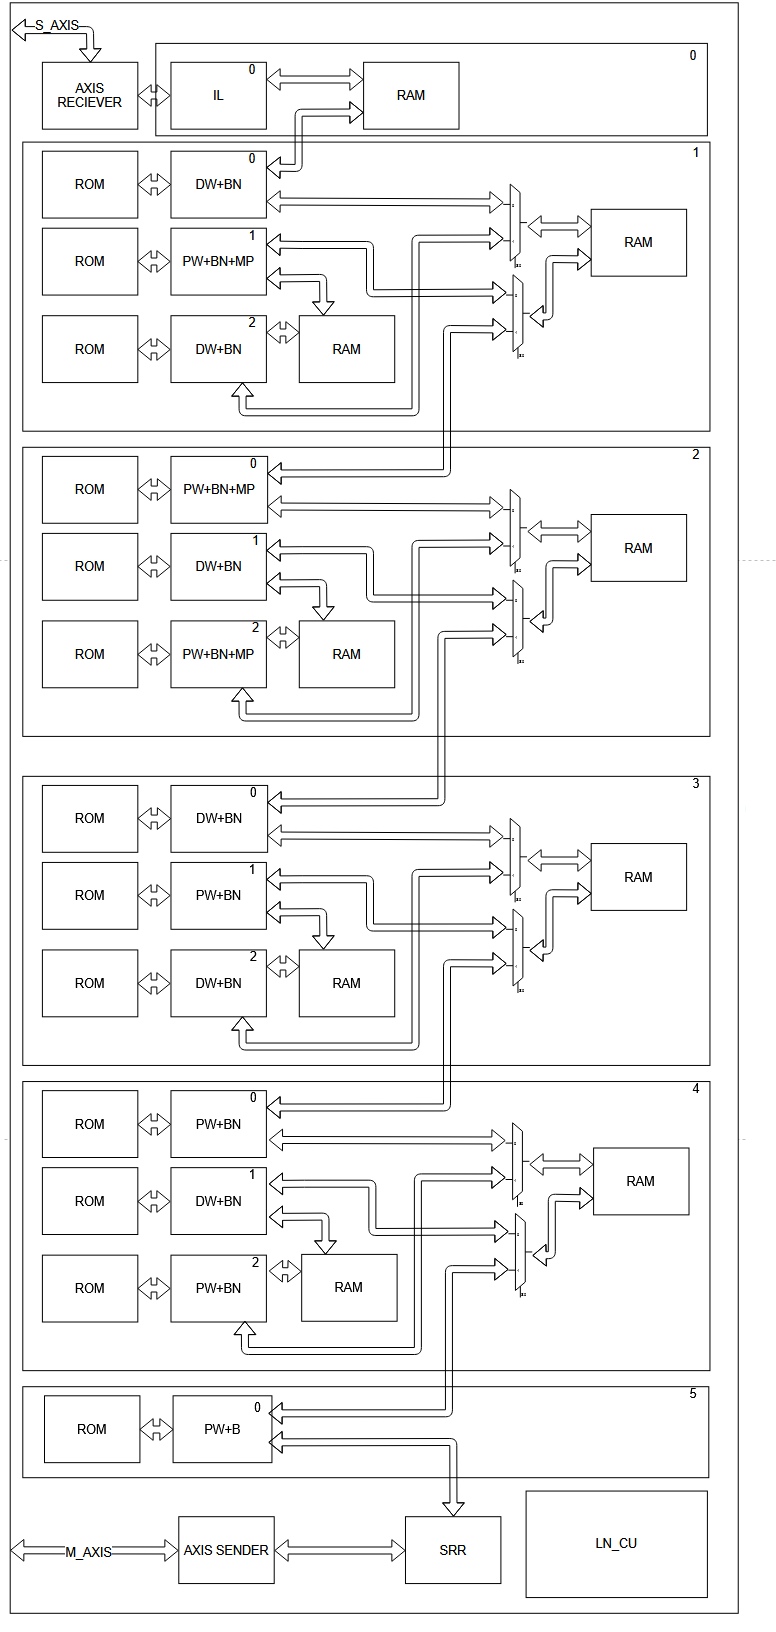
\includegraphics[height=0.9\textheight]{images/LNACC.png}
    \caption{Schemat akceleracji architektury \emph{LittleNet}. Uwzględniono jedynie najistotniejsze elementy.}
    \label{fig:LNACC}
\end{figure}
\begin{table}
    \centering
    \caption{Schemat aktywacji akceleratorów zrealizowany jako maszyna stanów.}
    \label{tab:LNACC}
    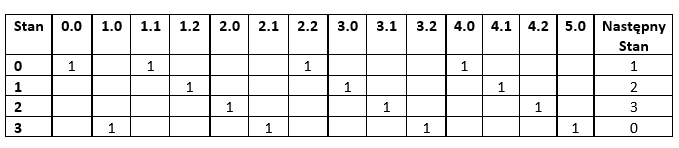
\includegraphics[width=0.9\textwidth]{images/acc_activ.png}
\end{table}

Wyróżniono 3 typy akceleratorów (dostępnych w~kilku konfiguracjach):
\begin{description}
\item warstwa wejściowa (IL),
\item warstwa \emph{depthwise} (DW),
\item warstwa \emph{pointwise} (PW).
\end{description}

Akceleratory warstw \emph{PW} pozwalają na równoległe wykonanie operacji.
Jednakże wymagany jest zapis do jednej pamięci w sposób szeregowy.
Do tego celu  wykorzystywany jest moduł \emph{MWU} (ang. \emph{Memory Writer Unit}) przedstawiony na rysunku \ref{fig:mwu}.
Wykonuje on operacje analogiczne do rejestru równoległo-szeregowego (o $P$ kanałach wejściowych).
Równoległe kanały wejściowe $CH\_i$ $P$ są odpowiednio opóźniane. 
Każdy kanał $CH\_{i}$ przechodzi przez linię opóźniającą \emph{D} o~latencji równej indeksowi sygnału $i$.
Do każdego kanału przypisany jest licznik adresu $CHD\_i$.
W przypadku, gdy opóźniona wartość kanału jest uznawana za ważną (ang. \emph{valid}) następuje inkrementacja adresu.
Wszystkie opóźnione kanały są multipleksowane przez moduł \emph{MUX}, wybierając kolejne kanały.
Wartość wybranego kanału wraz z opowiadającym adresem stanowią interfejs pamięci docelowej.
Ponadto dodatkowa logika sterująca została przedstawiona poprzez blok \emph{MW\_CU}(ang. \emph{Memory Writer Control Unit}).
\begin{figure}
    \centering
    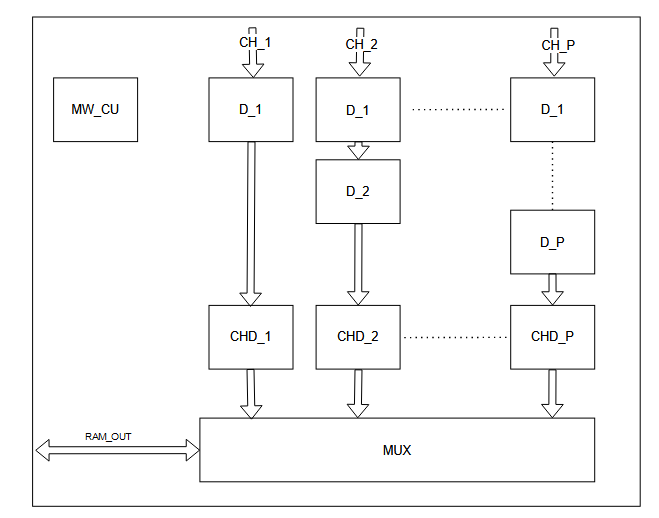
\includegraphics[width=0.8\linewidth]{images/MWU.png}
    \caption{\emph{MWU} -- schemat generowania adresu dla przetwarzania wielokanałowego.}
    \label{fig:mwu}
\end{figure}

\subsection{Warstwa wejsciowa}

Warstwa wejściowa \emph{IL} (ang. \emph{Input Layer}) realizuje zadanie zmiany formatu danych.
Schemat akceleratora został przedstawiony na rysunku \ref{fig:il}.
Dane wejściowe otrzymywane są w~notacji \emph{H-W-CH} (ang \emph{Height-Width-Channel}).
Na dalszym etapie przetwarzania wymagany jest format \emph{CH-H-W}.
Realizowane jest to poprzez buforowanie 3 kolejnych 32 bitowych pakietów danych w~rejestrze szeregowo-równoległym \emph{SPR}.
Zgromadzone dane są rozdzielane na poszczególne kanały \emph{R-G-B} (ang. \emph{Red-Green-Blue}) składając się na 32 bitowe pakiety po jednym na każdy kanał.
Uzyskany podział jest zapisywany do pamięci poprzez moduł \emph{MWU} dla 3 kanałów.
\begin{figure}
    \centering
    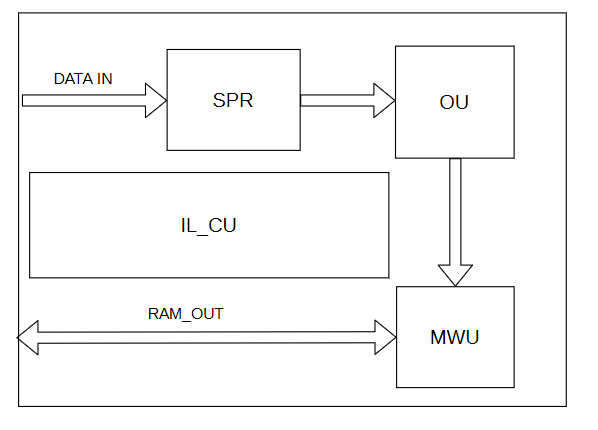
\includegraphics[width=0.8\linewidth]{images/ILACC.png}
    \caption{Schemat warstwy wejściowej \emph{IL}.}
    \label{fig:il}
\end{figure}

\subsection{Warstwa \emph{depthwise (DW)}}

Akceleracja konwolucji \emph{DW} jest realizowana razem z~warstwą normalizującą.
Na rysunku \ref{fig:dwacc} przedstawiono schemat akceleratora \emph{DW}.
Obliczenia wykonywane są w~architekturze potokowej drobnoziarnistej (ang. \emph{fine grained}). 
W tym celu moduł \emph{SWU} (ang. \emph{Sliding Window Unit}) generuje strumień danych wraz z~odpowiednimi opóźnieniami tak, aby uzyskać kontekst okna przesuwnego o~wymiarach 3x3.
Wykonanie operacji konwolucji wymaga wcześniejszego (przed rozpoczęciem strumieniowania każdego kanału) wczytania wag maski konwolucji.
Operację tę wykonuje moduł \emph{WSL} (ang. \textit{Weights Loading Unit}).
Sama operacja iloczynu skalarnego wektora wag i~kontekstu jest wykonywana przez \emph{DW\_PU} (ang. \emph{DepthWise Processing Unit}) przedstawiony na schemacie \ref{fig:dwpu}.
Wykorzystano tutaj możliwość kaskadowego połączenia kolejnych 9 \emph{DSP}. 
Dostępna jest konfiguracja wykorzystująca składową bias konwolucji (\emph{B}) oraz normalizację poprzez przekształcenie afiniczne (\emph{BN}).
Wynik konwolucji oraz normalizacji jest ograniczany (\emph{LIMIT}) do wartości wynikających z~wybranej notacji stałoprzecinkowej, czy też zastosowania funkcji $ReLU$.

Uzyskany rezultat jest zapisywany pod adresem wyznaczonym przez \emph{MWU}.
Sterowanie procesem akceleracji odbywa się poprzez logikę reprezentowaną przez \emph{DW\_CU} (ang. \emph{DepthWise Control Unit}).
Wykonanie wielokrotnej konwolucji \emph{DW} odbywa się poprzez wielokrotne (cykliczne) generowanie strumienia danych wejściowych przez \emph{SWU}.
\begin{figure}
    \centering
    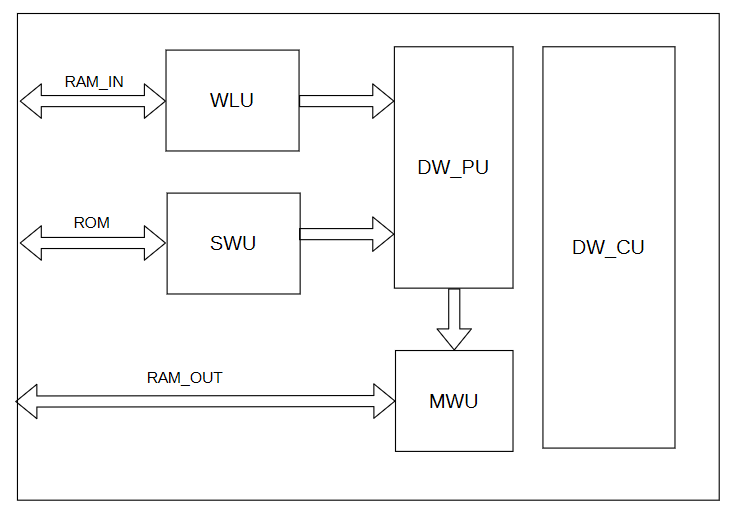
\includegraphics[width=0.9\linewidth]{images/DWACC.png}
    \caption{Schemat akceleratora \emph{DW} dostępnego w~wielu konfiguracjach.}
    \label{fig:dwacc}
\end{figure}
\begin{figure}
    \centering
    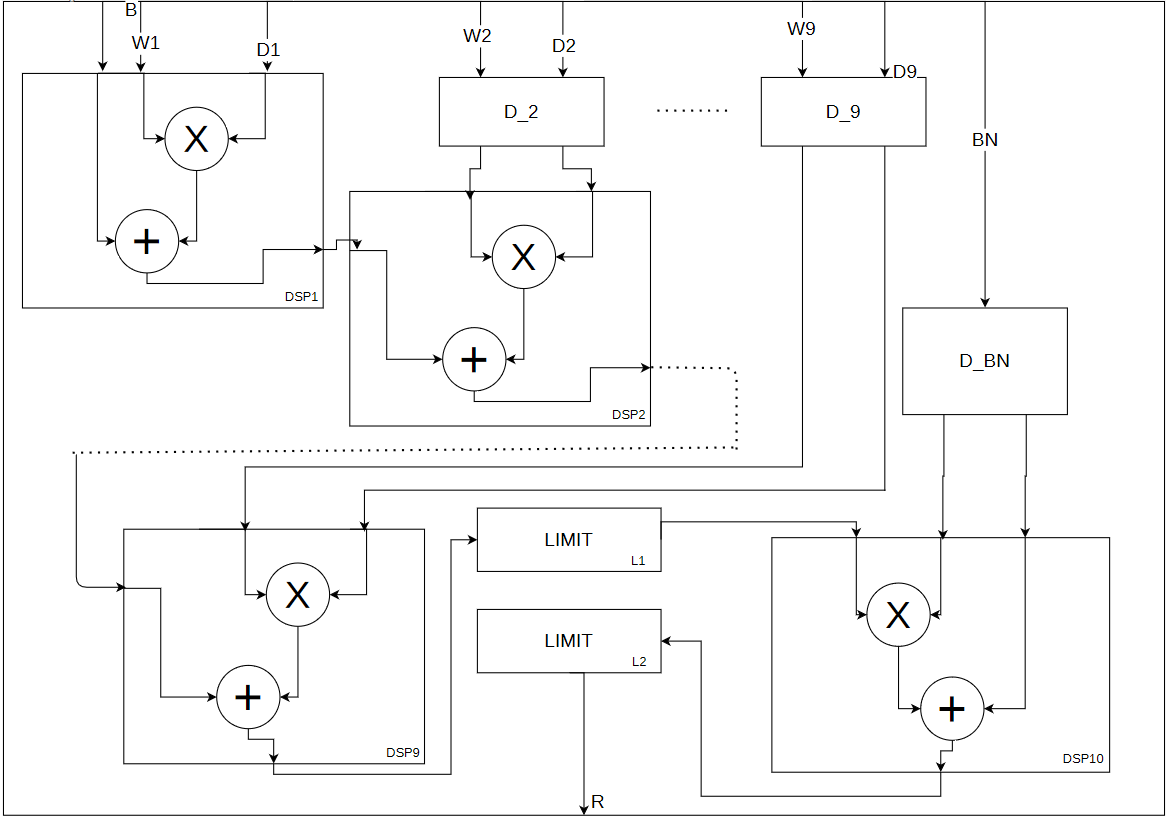
\includegraphics[width=0.9\linewidth]{images/DW_PU.png}
    \caption{Schemat \emph{DW\_PU} -- kaskadowe połączenie \emph{DSP}.
    Bloki \emph{DSP10+L2} są opcjonalne zależnie od konfiguracji.}
    \label{fig:dwpu}
\end{figure}

\subsection{Warstwa \emph{pointwise (PW)}}

Podobnie jak w~poprzednim przypadku akcelerator konwolucji \emph{PW} dostępny jest w~wielu konfiguracjach.
Schemat akceleratora \emph{PW} prezentuje rysunek \ref{fig:pwacc}.
Operacja konwolucji \emph{PW} nie wymaga gromadzenia otoczenia rozpatrywanego punktu, lecz iterowania po kolejnych kanałach wejściowych w~danym punkcie.
Jest to realizowane przez moduł \emph{PSU} (ang. \emph{Point Streamer Unit}).
Dla każdego kanału rozważanego punktu jest wymagana odpowiednia waga.
Ponadto identyczna sekwencja wag jest powtarzana dla następnych puntów.
W tym celu moduł \emph{CSU} (ang. \emph{Cyclic Streamer Unit}) generuje strumień w~sposób cykliczny.
Następuje wielokrotny odczyt z~kolejnych adresów zadanej puli adresowej definiowanej przez liczbę wag filtru. 
Przed rozpoczęciem generowania strumienia danych, odczytywane są wagi bias oraz przekształcenia afinicznego, które następnie są przechowaniem w~odpowiednich rejestrach.
Obliczenie konwolucji dla kolejnych punktów jest realizowane przez moduł \emph{PW\_PU} (ang. \emph{PointWise Processing Unit}) (rysunek \ref{fig:pwpu}).
Wykorzystuje się do tego celu operacje akumulacji z~mnożeniem.
Zakumulowana suma iloczynów jest (zależnie od konfiguracji) powiększana o~wartość bias.
Uzyskany rezultat zostaje ograniczony (identycznie jak w~konwolucji \emph{DW}).
W następnym kroku wykonywana jest operacja normalizacji wraz z~ponownym ograniczeniem wartości.

Następnym etapem przetwarzania jest (ewentualna) operacja \emph{Max Pooling}.
Do tego celu wykorzystuje się odpowiednie opóźnienia oraz porównywania wartości.
Uzyskany rezultat jest zapisywany pod adresem wyznaczanym przez moduł \emph{MWU}.
Opcjonalną funkcjonalnością (dla warstwy \emph{YOLOv3}) jest zastąpienie \emph{MWU} przez \emph{MFU} (ang. \emph{Max Finder Unit}) pozwalającego znaleźć punkt o~największej wartości (funkcja \emph{argmax}) wykrywalności obiektu, a~także zwrócić jego parametry (funkcja \emph{max}).
Ponadto istnieje możliwość zrównoleglenia obliczeń poprzez wykorzystanie $P$ modułów \emph{PW\_PU}. 
Wymaga to zastosowania pamięci ROM $P$-krotnie szerszej. 
Sterowanie poszczególnymi modułami jest zaimplementowane w bloku \emph{PW\_CU} (ang. \emph{PointWise Control Unit}).

\begin{figure}
    \centering
    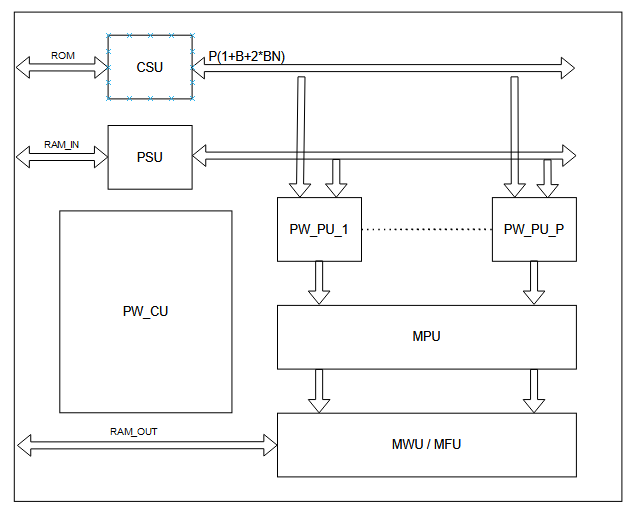
\includegraphics[width=0.9\linewidth]{images/PWACC.png}
    \caption{Schemat akceleratora \emph{PW} dostępnego w~wielu konfiguracjach.
    Opcjonalne są moduły \emph{MPU} oraz \emph{MWU} lub \emph{MFU}.}
    \label{fig:pwacc}
\end{figure}
\begin{figure}
    \centering
    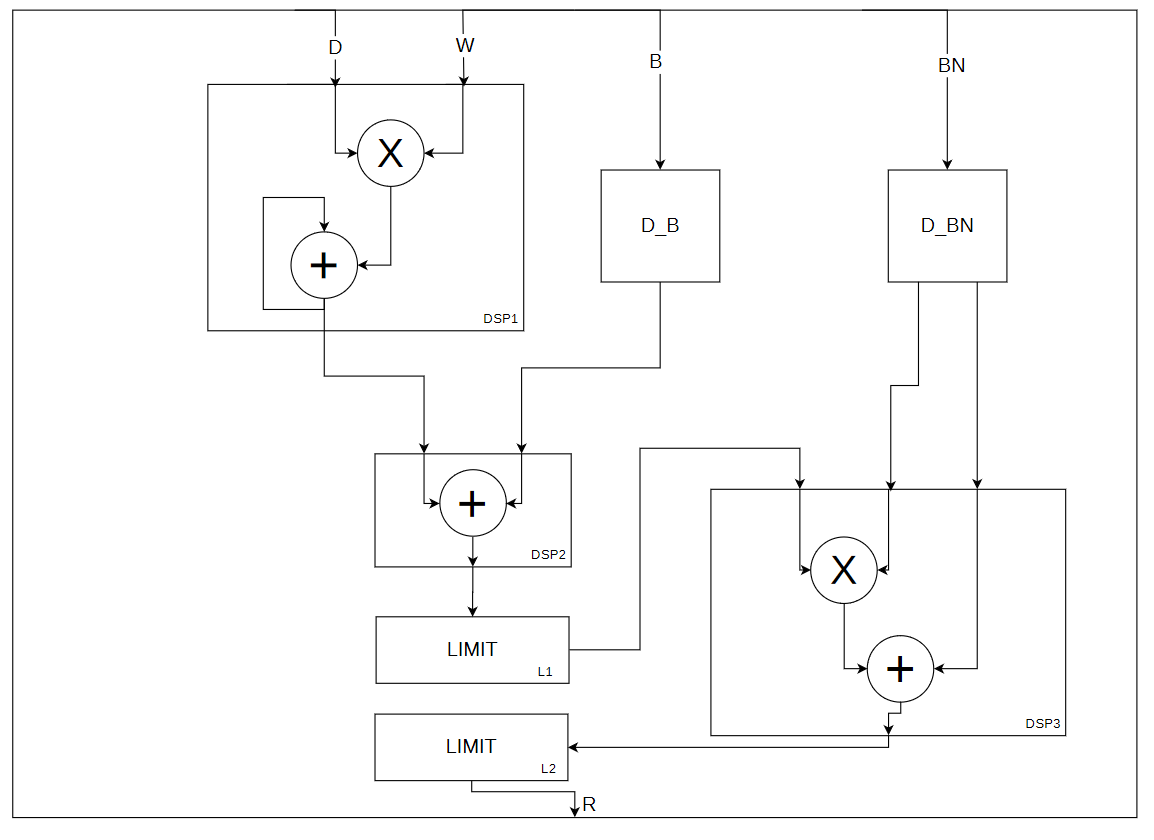
\includegraphics[width=0.8\linewidth]{images/PW_PU.png}
    \caption{Schemat \emph{PW\_PU} -- akumulacja z~mnożeniem realizowane przez \emph{DSP}. Bloki \emph{DSP2} oraz \emph{DSP3+L2} są opcjonalne i~zależne od konfiguracji.}
    \label{fig:pwpu}
\end{figure}

\subsection{Sterowanie akceleracją}

\label{ch:sterowanie}
Zaimplementowany akcelerator sieci \emph{LittleNet} został dołączony do schematu blokowego dostarczonego przez organizatorów konkursu.
Zmodyfikowany schemat przedstawiono na rysunku \ref{fig:vivado}. 
\begin{figure}
    \centering
    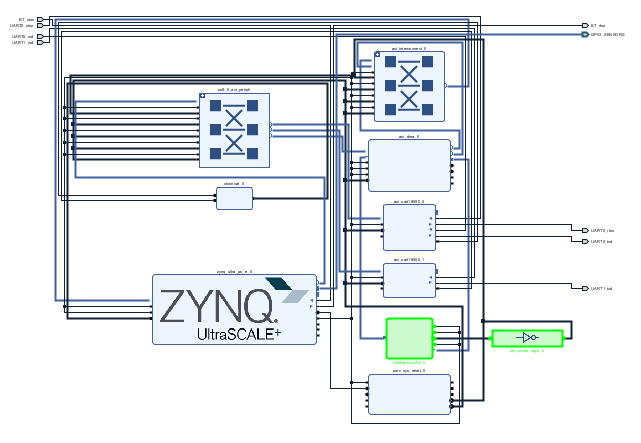
\includegraphics[width=0.9\linewidth]{images/vivado.png}
    \caption{Schemat blokowy w~środowisku \emph{Vivado 2019.1}. Zaznaczono dodane elementy -- akcelerator oraz negacja sygnału \emph{reset}.}
    \label{fig:vivado}
\end{figure}

Uzyskaną modyfikacją poddano syntezie, implementacji oraz wygenerowano plik \emph{bit} w~środowisku \emph{Vivado 2019.1} dostarczonym przez firmę \emph{Xilinx}.
Otrzymane rezultaty (pliki \emph{*.hwh} oraz \emph{*.bit}) umieszczono w~odpowiednio skonfigurowanym środowisku na platformie \emph{Avnet Ultra96 V2}.
Aplikacje sterującą zrealizowano w~postaci notatnika \emph{Jupyter}.
Konfiguracja logiki programowalnej oraz przesył danych do oraz z~akceleratora zostały zrealizowane z~użyciem biblioteki \emph{PYNQ}. 
Odczyt obrazów oraz przetwarzanie rezultatów zaimplementowano w~sposób równoległy do procesu akceleracji.
Analizując dokładniej schemat akceleracji można zauważyć, iż rezultat przetwarzania danego obrazu jest uzyskiwany po 4 cyklach przetwarzania.
Wymaga to odrzucenia początkowych rezultatów oraz wykonania dodatkowych cykli akceleracji, aby uzyskać poprawny wynik dla wszystkich obrazów wejściowych.


\section{Podsumowanie}
Przeprowadzony proces implementacji wymagał na początkowym etapie wyznaczenia modelu programowego. 
W tego celu wykorzystano biblioteką \emph{PyTorch} oraz \emph{Brevitas}.
Pierwszy etap wymagał wytrenowania modelu zmiennoprzecinkowego.
Uzyskany model zastał następnie poddany odpowiedniej kwantyzacji.
Zrealizowanie sprzętowej akceleracji wymagało opracowania sposobu implementacji poszczególnych warstw, jak i~całej sieci.
Wyszczególniono 3 typy akceleratorów: warstwa wejściowa,  \emph{DW} oraz \emph{PW}.
Pierwsza z~wymienionych dokonuje zmiany formatu danych wejściowych.
Pozostałe dwie warstwy realizuję odpowiednie konwolucje wraz z~normalizacją.
Warstwa \emph{PW} możliwa jest do konfiguracji realizującej operacje \emph{Max Pooling} czy też funkcji \emph{argmax} oraz \emph{max}. 
Możliwe jest także dodatkowe zrównoleglenie poprzez wykorzystanie większej liczby modułów \emph{PW\_PU}. 
Akceleracja całej sieci oparta jest o~architekturę potokową gruboziarnistą z~opóźnieniem 4 cykli przetwarzania.
Zastosowanie akceleratora do przetwarzania obrazów wymagało implementacji z~wykorzystaniem notatnika \emph{Jupyter} możliwego do modyfikacji w~trakcie ewaluacji. 













	\chapter{Ewaluacja sprzętowa i optymalizacja}
\label{cha:Optymalizacja}
% Ewaluacja po implementacji sprzętowej. 
% Optymalizacja fps / energii.

% Wyznaczony model sieci \emph{LittleNet} w rozdziale \cite{ch:LN} został zaimplementowany sprzętowo co zostało omówione w  
W rozdziale \ref{ch:LN} wyznaczono model sieci \emph{LittleNet}. 
Architektura ta osiąga wartość $IoU = 0.71$ (dla zbioru testowego). 
Sieć została zaimplementowana sprzętowo co omówiono w rozdziale \ref{cha:Implementacja}.
Rozwiązanie to jednak należy sprawdzić pod kątem dokładności detekcji (poprawności z modelem programowym), przepustowości oraz zużycia energii, a także dokonać próby optymalizacji ich optymalizacji. 


\section{Ewaluacja}
Celem sprawdzenia zaprojektowanego rozwiązania wykorzystano zaimplementowaną aplikację sterującą (rozdział \ref{ch:sterowanie}).
Aplikacja pozwala na pomiar czasu przetwarzania oraz pomiar energii.
Aby możliwe było sprawdzenie dokładności otrzymanych rezultatów zaimplementowano funkcję obliczającą wartość metryki $IoU$ względem wartości referencyjnych.

Wstępne wyniki ewaluacji dawały inne rezultaty niż model programowy.
Dalsza analiza pozwoliła stwierdzić, iż model programowy wykorzystywał operacje zmiennoprzecinkowe do przeskalowania rozmiaru obrazu wejściowego.
Wykorzystanie do tego celu liczb całkowitych nieznacznie pogorszyło wynik.
Finalnie oba modele dawały identyczne rezultaty w postaci $IoU = 0.7015$, 
Wykorzystano tutaj ośmiokrotne zrównoleglenie warstw \emph{PW} pozwalające na osiągnięcie średnich wartości przepustowości $fps = 52.5$ oraz zużycia energii $e = 3652 J$ (wartość dla $52 500$ obrazów). 
Uzyskana dokładność oraz przepustowość pozwalają na osiągnięcie maksymalnych wartości funkcji \eqref{eq:iou_score} oraz \eqref{eq:fps_score}.
Na rysunku \ref{fig:results} przedstawiono rezultaty detekcji dla wybranych obrazów wchodzących w skład zbioru testowego.

\begin{figure}
    \centering
    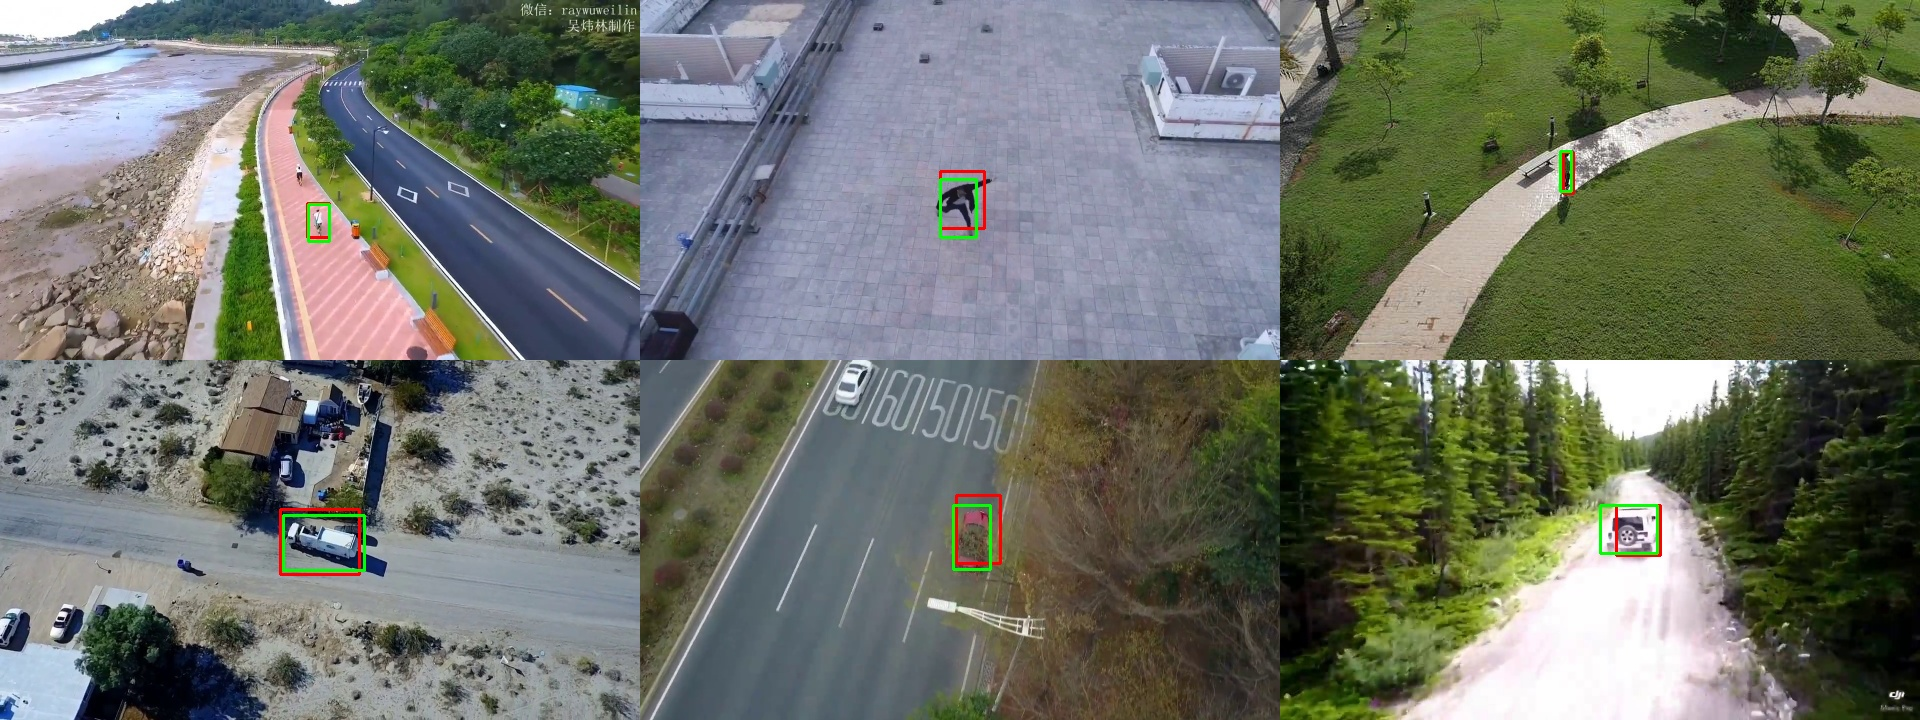
\includegraphics[width=0.9\linewidth]{images/results.png}
    \caption{Uzyskane rezultaty detekcji dla wybranych obrazów zbioru uczącego. 
    Źródło: \cite{dac_sdc_2021}.}
    \label{fig:results}
\end{figure}

\section{Optymalizacja}
Zakładając, iż otrzymana dokładność detekcji została by osiągnięta na zbiorze tajnym, optymalizacja może zostać ograniczona jedynie zmian parametrów akceleracji, takich jak zrównoleglenie $p$ warstw \emph{PW} czy częstotliwość zegara $f$ dla logiki programowalnej (dotychczas używana była częstotliwość $100$ MHz).
Łączną moc układu można wyrazić wzorem \eqref{eq:power}, gdzie $P_{PL}(p,f)$ to moc logiki programowalnej oraz $P_{PL}(p,f)$ moc układu procesorowego.
\begin{equation}
P(p,f) = P_{PS} + P_{PL}(p,f)
\label{eq:power}
\end{equation}
Zużycie energii $e$ układu potrzebnej do przeprowadzenia procesu detekcji $N$ obrazów osiągające przepustowość $fps(p,f)$ definiuje równanie \eqref{eq:energy}.
\begin{equation}
e(p,f) = \frac{N}{fps(p,f)}(P_{PS} + P_{PL}(p,f))
\label{eq:energy}
\end{equation}

Ponadto przybliżoną moc $P_{PL}(p,f)$ wyrazić można przez \eqref{eq:ppl}, zakładając liniowy przyrost mocy od $p$ dla warstw \emph{PW} oraz zależność mocy od częstotliwości przyjmując za $\beta(f)$. Przez $P_{DW}$ oraz $P_{PW}$ oznaczono moc akceleratorów odpowiednio \emph{DW} i \emph{PW} (dla akceleracji z użyciem tylko jednego \emph{PW\_PU}).
\begin{equation}
P_{PL}(p,f) = \beta(f) (P_{DW} + p P_{PW})
\label{eq:ppl}
\end{equation}

Przybliżony stosunek czasu trwania obliczeń warstwy \emph{DW} do czasu trwania całego cyklu przetwarzania wyrażono poprzez $\alpha(p)$. 
Wartości stałe stanowią liczbę maksymalnych wymaganych odczytów z pamięci RAM dla  warstw \emph{PW}(10 444 800) oraz \emph{DW}(460 000).
\begin{equation}
\alpha(p) = \frac{460 000}{460 000 + \frac{10 444 800}{p}} = \frac{p}{p+22.7}
\label{eq:alpha}
\end{equation}

Z równia \eqref{eq:alpha} można stwierdzić, iż znaczna część czasu przetwarzania przypada na akcelerację warstw \emph{PW} ($\alpha(1) = 0.04$, $\alpha(8) = 0.26$,  $\alpha(16) = 0.41$).
Tym samym zakładając \eqref{eq:fps}, gdzie $f_0$ oraz $fps_0$ to stałe.
\begin{equation}
fps(p,f) = p*\frac{f}{f_0}* fps_0
\label{eq:fps}
\end{equation}

Równanie zużycia energii przybiera postać \eqref{eq:energy_simple}.
\begin{equation}
e(p,f) = \frac{N}{p*\frac{f}{f_0}* fps_0}(P_{PS} + \beta (f) P_{DW} + p \beta (f) P_{PW})
\label{eq:energy_simple}
\end{equation}

Przyjmując $f$ jako stałą oraz zrównoleglenie $p_1$ oraz $p_2$ takie, że $p_1 < p_2$ 
to stosunek zużytej energii $e_2$ dla  $p_2$ do zużytej energii $e_1$ dla  $p_1$ wyznaczany jest przez \eqref{eq:e_cmp}.
\begin{equation}
\begin{aligned}
\frac{e_2}{e_1} = \frac{e(p_2)}{e(p_1)} &= \frac
{\frac{1}{p_2}(P_{PS} + \beta(f) P_{DW} + p_2 \beta(f) P_{PW})}
{\frac{1}{p_1}(P_{PS} + \beta(f) P_{DW} + p_1 \beta(f) P_{PW})}\\
&= \frac
{\frac{C_1}{p_2} + C_2}
{\frac{C_1}{p_1} + C_2}
\end{aligned}
\label{eq:e_cmp}
\end{equation}
 Większe zrównoleglenie przyniesie mniejsze zużycie energii, gdy $\frac{e_2}{e_1} < 1$ co jest prawdziwe dla każdego $p_2 > p_1$. 
 Wnioskując im wyższy stopnień zrównoleglenia tym mniejsze zużycie energii.
 W tym celu ustalono $p = 16$ oraz przeprowadzono ewaluacje.
 W rezultacie uzyskano $fps = 72.7$ oraz zużycie energii $e = 2739 J$.
 Co jest zgodne z wyznaczonymi nierównościami, pomimo zastosowania znacznych przybliżeń.
 
 Dla \eqref{eq:energy_simple} przyjmując $p$ jako stałą oraz przyjmując $P_{PL}$ jako moc dynamiczną bez straty ogólności (nie znana jest moc $P_{PS}$), wówczas zależność mocy od częstotliwości może zostać wyrażona poprzez \eqref{eq:dynf} \cite{dynamic_power} oraz zużycie energii poprzez \eqref{eq:energy_simple_f}. 
\begin{equation}
\beta(f) = \frac{f}{f_0}
\label{eq:dynf}
\end{equation} 
\begin{equation}
e(p,f) = \frac{N}{p*\frac{f}{f_0}* fps_0}(P_{PS} + \frac{f}{f_0} P_{PL})
\label{eq:energy_simple_f}
\end{equation}

Przyjmując dwie częstotliwości $f_1$ oraz $f_2$ takie, że $f_2 > f_1$, możliwe jest zmniejszenie zużycia energii, gdy spełniona jest zależność \eqref{eq:cmp}.
\begin{equation}
e(p, f_2) < e(p,f_1)
\label{eq:cmp}
\end{equation}
\begin{equation}
\frac{1}{f_2}(P_{PS} + \frac{f_2}{f_0} P_{PL}) < 
\frac{1}{f_1}(P_{PS} + \frac{f_1}{f_0} P_{PL})
\end{equation}
\begin{equation}
\frac{P_{PS}}{f_2} < 
\frac{P_{PS}}{f_1}
\end{equation}
\begin{equation}
f_1 < f_2
\end{equation}
co jest zawsze prawdziwe.
Wnioskując im większa częstotliwość przetwarzania, tym mniejsze zużycie energii.
Wartość częstotliwości musi jednak zapewniać prawidłowe wykonanie obliczeń.
Ponadto niejawnie zakładano, iż część przetwarzania realizowana przez procesor będzie wykonana w czasie krótszym, niż obliczenia logiki programowalnej.
Eksperymentalnie sprawdzono, iż maksymalna częstotliwość pracy akceleratora nie może być większa niż 215 MHz.
Obecna implementacja programowa nie pozwoliła jednak na uzyskanie wyższej przepustowości niż dotychczas.Dla wspomnianej maksymalnej częstotliwości uzyskano $fps = 71.0$ oraz zużycie energii $e = 2798 J$.

Aby sprawdzić zużycie energii wynikające z pracy akceleratora, postanowiono pominąć etap odczytu danych oraz późniejszego przetwarzania z użyciem systemu procesorowego.
Uzyskano wówczas $fps = 183 $ oraz $e = 1070 J$, co dowodzi słuszności wcześniejszych rozważań.
 
 
\begin{figure}
    \centering
    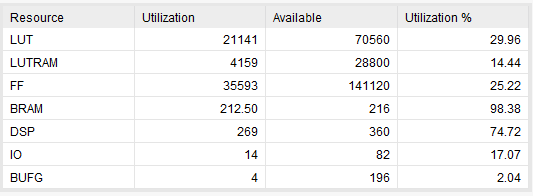
\includegraphics[width=0.9\linewidth]{images/zasoby.png}
    \caption{Zużycie zasobów - zrzut ekranu z programu \emph{Vivado 2019.1}.}
    \label{fig:resources}
\end{figure}
Ostateczne rozwiązanie zostało zaimplementowane ze zrównolegleniem $p = 16$.
Na rysunku \ref{fig:resources} przestawiono zużycie zasobów logiki programowalnej.
Implementacja wykorzystuje niemal wszystkie bloki pamięci \emph{BRAM} oraz znaczą część dostępnych \emph{DSP}.
Uzyskanie ostatecznie lepszych rezultatów jest możliwe, jedynie poprzez bardziej wydajną implementację części programowej.




	\chapter{Podsumowanie}
\label{cha:Podsumowanie}

% Porównanie rezultatów(narzędzia, kwantyzacje itp.).
% Jeżeli to będzie po ogłoszeniu wyników to wyniki konkursu.

W ramach niniejszej pracy przedstawiono proces projektowania architektury sieci neuronowej do detekcji obiektów, która została następnie zaimplementowana na platformie sprzętowo-programowej Zynq UltraScale+ MPSoC.
System ten był opracowywany na potrzeby konkursu \emph{2021 DAC SDC}. 
% W tym celu wymagane było dokładne przeanalizowanie wymagań, a~także zapoznanie z~docelową platformą -- płytką rozwojową \emph{Avnet Ultra96 V2}. 
% Przedstawiono również dostępne narzędzia pozwalające na przejście z~modelu zmiennoprzecinkowego, przez model kwantyzowany, aż do sprzętowej akceleracji.
% Zaproponowanie własnego rozwiązania problemu detekcji wymagało rozeznania się w~już istniejących. 
% W tym celu dokonano przeglądu literatury przedstawiając zarówno rozwiązania klasyczne, jak i~te wykorzystujące głębokie sieci neuronowe. 
Analizując stawiane wymagania, parametry docelowej platformy sprzętowej, a także rozwiązania z poprzednich edycji zaproponowano architekturę sieci \emph{LittleNet}.
Zastosowano konwwolucje \emph{depthwise} wykorzystującą wielu filtrów dla każdego kanału oraz konwolucje \emph{pointwise}.
Rozwiązanie to osiągało dokładność $IoU = 0.78$ dla modelu zmiennoprzecinkowego.
Przejście przez etap kwantyzacji do zapisu stałoprzecinkowego pozwoliło uzyskać już wartość $IoU = 0.7015$ (przy skalowaniu obrazu z~wykorzystaniem liczb całkowitych).
Wartość ta niestety tylko w niewielkim stopniu przekracza próg pozwalający na osiągnięcie maksymalnej wartości funkcji oceny dokładności detekcji.
Zdecydowano się na zaprojektowanie własnego akceleratora sprzętowego z~wykorzystaniem języka \emph{System Verilog}. 
Moduł, po przeprowadzonej optymalizacji, osiągał przepustowość rzędu $72.7 fps$ zużywając $2739 J$ energii.
Możliwa jest praca przy częstotliwości nawet $215$ MHz osiągając przepustowość $183 fps$ oraz zużycie energii wynoszące $1070 J$. 
Jednakże wynik ten uzyskiwany był z~pominięciem odczytu obrazów oraz wszelkiego przetwarzania z~użyciem systemu procesorowego.
Zatem na obecnym etapie ''wąskim gardłem'' jest niewydajna implementacją programowa
i~opisany powyżej zabieg nie ma uzasadnienia.

Zaimplementowane rozwiązanie pozwala na osiągnięcie dobrych rezultatów. 
Jednakże, aby możliwe było poprawienie wydajności niezbędne jest zaimplementowanie części programowej w~sposób wydajny np. wykorzystując język \emph{C} wraz z~przetwarzaniem wielowątkowym.
Na etapie uczenia zastosowano funkcję \emph{GCIoU} \eqref{eq:gciou}, której rezultaty należy jeszcze porównać z innymi funkcjami bazującymi na metryce \emph{IoU}.
Możliwe jest również zwiększenie dokładności obliczeń poprzez zmniejszenie stopnia kwantyzacji (zapis wykorzystujący więcej bitów) czy też uzależnienie go od konkretnych warstw (różna kwantyzacja dla warstw).
Ponadto możliwe jest zredukowanie rozmiaru sieci, poprzez usunięcie wybranych filtrów tzw. \emph{pruning}.
Dobór liczby bitów części całkowitej można spróbować zrealizować w sposób automatyczny, poprzez ustanowienie jako parametr podlegający uczeniu.
Zaproponowane typy akceleratorów można również poszerzyć m.in. o~operację pełnej konwolucji, czy warstwy \emph{FC}.
Ponadto proces uczenia sieci można zrealizować np. z~użyciem klastra obliczeniowego \emph{Prometeusz} z \emph{Akademickiego Centrum
Komputerowego CYFRONET}.
%, tym samym pozbywając rezygnując z limitów usługi \emph{GoogleColab}.

	% itd.
	% \appendix
	% \include{dodatekA}
	% \include{dodatekB}
	% itd.
	
	\printbibliography

\end{document}
